\documentclass[13 pt,]{book}
\usepackage{lmodern}
\usepackage{amssymb,amsmath}
\usepackage{ifxetex,ifluatex}
\usepackage{fixltx2e} % provides \textsubscript
\ifnum 0\ifxetex 1\fi\ifluatex 1\fi=0 % if pdftex
  \usepackage[T1]{fontenc}
  \usepackage[utf8]{inputenc}
\else % if luatex or xelatex
  \ifxetex
    \usepackage{mathspec}
  \else
    \usepackage{fontspec}
  \fi
  \defaultfontfeatures{Ligatures=TeX,Scale=MatchLowercase}
    \setmonofont[Mapping=tex-ansi,Scale=0.7]{Source Code Pro}
\fi
% use upquote if available, for straight quotes in verbatim environments
\IfFileExists{upquote.sty}{\usepackage{upquote}}{}
% use microtype if available
\IfFileExists{microtype.sty}{%
\usepackage{microtype}
\UseMicrotypeSet[protrusion]{basicmath} % disable protrusion for tt fonts
}{}
\usepackage[margin=1in]{geometry}
\usepackage{hyperref}
\hypersetup{unicode=true,
            pdftitle={South Asia Micro Database (SARMD) User Guidelines},
            pdfauthor={South Asia Region Team for Statistical Development (SARTSD)},
            pdfborder={0 0 0},
            breaklinks=true}
\urlstyle{same}  % don't use monospace font for urls
\usepackage{natbib}
\bibliographystyle{apalike}
\usepackage{color}
\usepackage{fancyvrb}
\newcommand{\VerbBar}{|}
\newcommand{\VERB}{\Verb[commandchars=\\\{\}]}
\DefineVerbatimEnvironment{Highlighting}{Verbatim}{commandchars=\\\{\}}
% Add ',fontsize=\small' for more characters per line
\usepackage{framed}
\definecolor{shadecolor}{RGB}{248,248,248}
\newenvironment{Shaded}{\begin{snugshade}}{\end{snugshade}}
\newcommand{\KeywordTok}[1]{\textcolor[rgb]{0.13,0.29,0.53}{\textbf{{#1}}}}
\newcommand{\DataTypeTok}[1]{\textcolor[rgb]{0.13,0.29,0.53}{{#1}}}
\newcommand{\DecValTok}[1]{\textcolor[rgb]{0.00,0.00,0.81}{{#1}}}
\newcommand{\BaseNTok}[1]{\textcolor[rgb]{0.00,0.00,0.81}{{#1}}}
\newcommand{\FloatTok}[1]{\textcolor[rgb]{0.00,0.00,0.81}{{#1}}}
\newcommand{\ConstantTok}[1]{\textcolor[rgb]{0.00,0.00,0.00}{{#1}}}
\newcommand{\CharTok}[1]{\textcolor[rgb]{0.31,0.60,0.02}{{#1}}}
\newcommand{\SpecialCharTok}[1]{\textcolor[rgb]{0.00,0.00,0.00}{{#1}}}
\newcommand{\StringTok}[1]{\textcolor[rgb]{0.31,0.60,0.02}{{#1}}}
\newcommand{\VerbatimStringTok}[1]{\textcolor[rgb]{0.31,0.60,0.02}{{#1}}}
\newcommand{\SpecialStringTok}[1]{\textcolor[rgb]{0.31,0.60,0.02}{{#1}}}
\newcommand{\ImportTok}[1]{{#1}}
\newcommand{\CommentTok}[1]{\textcolor[rgb]{0.56,0.35,0.01}{\textit{{#1}}}}
\newcommand{\DocumentationTok}[1]{\textcolor[rgb]{0.56,0.35,0.01}{\textbf{\textit{{#1}}}}}
\newcommand{\AnnotationTok}[1]{\textcolor[rgb]{0.56,0.35,0.01}{\textbf{\textit{{#1}}}}}
\newcommand{\CommentVarTok}[1]{\textcolor[rgb]{0.56,0.35,0.01}{\textbf{\textit{{#1}}}}}
\newcommand{\OtherTok}[1]{\textcolor[rgb]{0.56,0.35,0.01}{{#1}}}
\newcommand{\FunctionTok}[1]{\textcolor[rgb]{0.00,0.00,0.00}{{#1}}}
\newcommand{\VariableTok}[1]{\textcolor[rgb]{0.00,0.00,0.00}{{#1}}}
\newcommand{\ControlFlowTok}[1]{\textcolor[rgb]{0.13,0.29,0.53}{\textbf{{#1}}}}
\newcommand{\OperatorTok}[1]{\textcolor[rgb]{0.81,0.36,0.00}{\textbf{{#1}}}}
\newcommand{\BuiltInTok}[1]{{#1}}
\newcommand{\ExtensionTok}[1]{{#1}}
\newcommand{\PreprocessorTok}[1]{\textcolor[rgb]{0.56,0.35,0.01}{\textit{{#1}}}}
\newcommand{\AttributeTok}[1]{\textcolor[rgb]{0.77,0.63,0.00}{{#1}}}
\newcommand{\RegionMarkerTok}[1]{{#1}}
\newcommand{\InformationTok}[1]{\textcolor[rgb]{0.56,0.35,0.01}{\textbf{\textit{{#1}}}}}
\newcommand{\WarningTok}[1]{\textcolor[rgb]{0.56,0.35,0.01}{\textbf{\textit{{#1}}}}}
\newcommand{\AlertTok}[1]{\textcolor[rgb]{0.94,0.16,0.16}{{#1}}}
\newcommand{\ErrorTok}[1]{\textcolor[rgb]{0.64,0.00,0.00}{\textbf{{#1}}}}
\newcommand{\NormalTok}[1]{{#1}}
\usepackage{longtable,booktabs}
\usepackage{graphicx,grffile}
\makeatletter
\def\maxwidth{\ifdim\Gin@nat@width>\linewidth\linewidth\else\Gin@nat@width\fi}
\def\maxheight{\ifdim\Gin@nat@height>\textheight\textheight\else\Gin@nat@height\fi}
\makeatother
% Scale images if necessary, so that they will not overflow the page
% margins by default, and it is still possible to overwrite the defaults
% using explicit options in \includegraphics[width, height, ...]{}
\setkeys{Gin}{width=\maxwidth,height=\maxheight,keepaspectratio}
\IfFileExists{parskip.sty}{%
\usepackage{parskip}
}{% else
\setlength{\parindent}{0pt}
\setlength{\parskip}{6pt plus 2pt minus 1pt}
}
\setlength{\emergencystretch}{3em}  % prevent overfull lines
\providecommand{\tightlist}{%
  \setlength{\itemsep}{0pt}\setlength{\parskip}{0pt}}
\setcounter{secnumdepth}{5}
% Redefines (sub)paragraphs to behave more like sections
\ifx\paragraph\undefined\else
\let\oldparagraph\paragraph
\renewcommand{\paragraph}[1]{\oldparagraph{#1}\mbox{}}
\fi
\ifx\subparagraph\undefined\else
\let\oldsubparagraph\subparagraph
\renewcommand{\subparagraph}[1]{\oldsubparagraph{#1}\mbox{}}
\fi

%%% Use protect on footnotes to avoid problems with footnotes in titles
\let\rmarkdownfootnote\footnote%
\def\footnote{\protect\rmarkdownfootnote}

%%% Change title format to be more compact
\usepackage{titling}

% Create subtitle command for use in maketitle
\newcommand{\subtitle}[1]{
  \posttitle{
    \begin{center}\large#1\end{center}
    }
}

\setlength{\droptitle}{-2em}

  \title{South Asia Micro Database (SARMD) User Guidelines}
    \pretitle{\vspace{\droptitle}\centering\huge}
  \posttitle{\par}
    \author{South Asia Region Team for Statistical Development (SARTSD)}
    \preauthor{\centering\large\emph}
  \postauthor{\par}
      \predate{\centering\large\emph}
  \postdate{\par}
    \date{2019-03-31}

\usepackage{booktabs}
\usepackage{amsthm}
\makeatletter
\def\thm@space@setup{%
  \thm@preskip=8pt plus 2pt minus 4pt
  \thm@postskip=\thm@preskip
}
\makeatother

\begin{document}
\maketitle

{
\setcounter{tocdepth}{1}
\tableofcontents
}
\chapter*{Preface}\label{preface}
\addcontentsline{toc}{chapter}{Preface}

\begin{center}\rule{0.5\linewidth}{\linethickness}\end{center}

\begin{figure}[htbp]
\centering
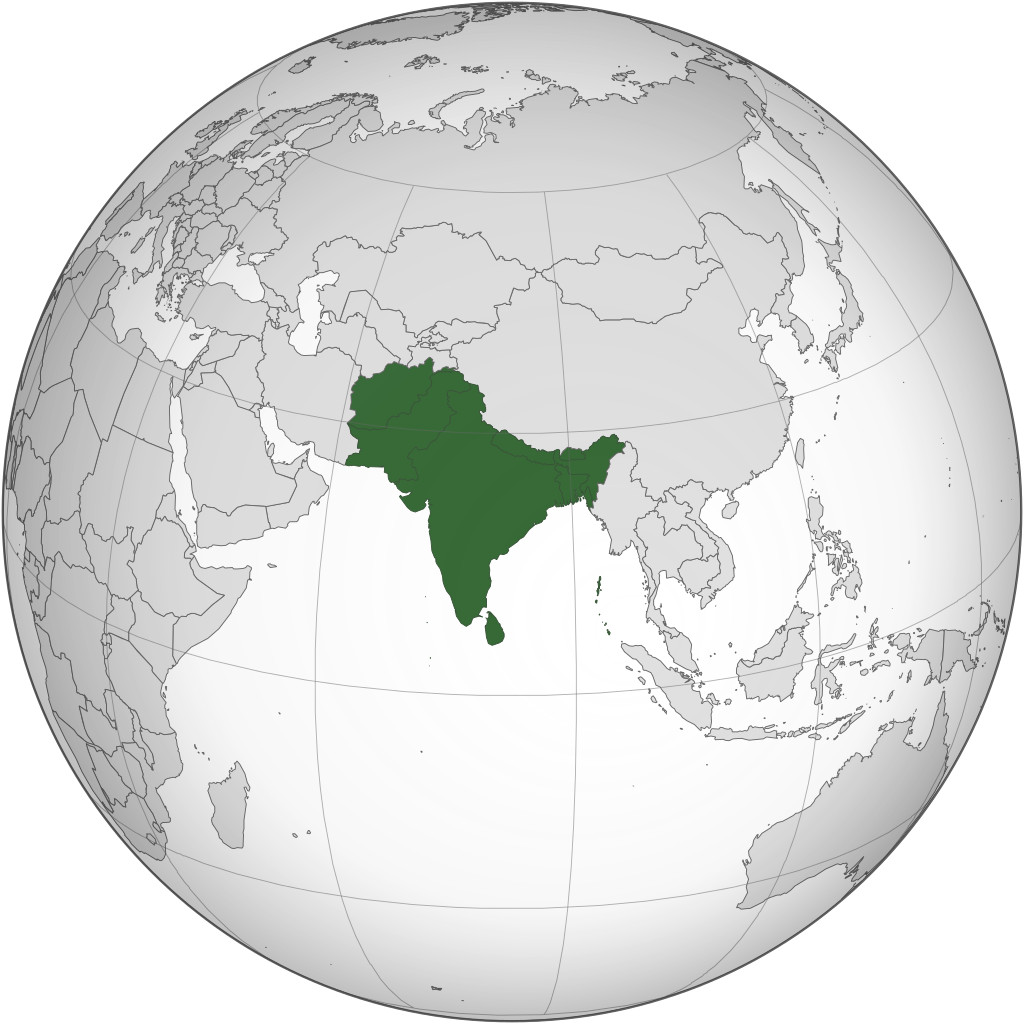
\includegraphics{figures/sarmap.png}
\caption{}
\end{figure}

\begin{center}\rule{0.5\linewidth}{\linethickness}\end{center}

These user guidelines provide help to any researcher interested in
working with regionally-comparable estimates of poverty incidence,
demographic characteristics, education, labor, and household welfare
provided by the South Asia Micro Database (SARMD). The region of South
Asia consists of eight countries (Afghanistan, Bangladesh, Bhutan,
India, Maldives, Nepal, Pakistan, and Sri Lanka) for which there is at
least satisfactory data availability. SARMD provides access to the
nationally representative cross-sectional household surveys that form
the basis to measure consumption-based poverty in South Asia. These
household surveys focus on households as both consuming and producing
units of analysis for which a nominal measure of total household
expenditures is constructed by adding four expenditure components:

\begin{enumerate}
\def\labelenumi{\roman{enumi}.}
\tightlist
\item
  food expenditures;
\item
  non-food, non-durable expenditures;
\item
  expenditures on durables; and
\item
  expenditures on housing.
\end{enumerate}

The main welfare measure used in the region to measure poverty, the
expenditures per capita aggregate, must be spatially and temporally
adjusted, and converted into 2011 purchasing power parity (PPP) dollars,
to be used to calculate the proportion of people below the extreme
poverty line of \$1.90 per person per day. According to the extreme
poverty headcounts in the
\href{http://www.worldbank.org/en/publication/poverty-and-shared-prosperity}{Poverty
and Shared Prosperity Report (2018)}, in 2015, South Asia accounted for
29\% of the estimated 736 million people living in extreme poverty
worldwide. Even though the region of South Asia does not lack data,
these poverty headcounts and other welfare measures rely on household
survey data that suffers from low frequency and comparability over time
and across countries. This book overviews how the content, length, and
complexity of the household surveys collected in the region vary between
countries, and even within countries over time. It then provides a guide
for the harmonization of variables across the region.

Harmonization facilitates the use of household data at a regional level,
especially when harmonized variables are constructed carefully. We
provide a few examples on how the harmonized variables in SARMD may be
used for research purposes. In the simple example below, household
access to at least one bicycle (Yes=1, No=0) is averaged at a
subnational (state or province) level and plotted in a map for the most
recent survey available in each country. Even though survey
characteristics vary and data comes from different years, having access
to a bicycle seems to be significantly more common for households in
Eastern India than in other areas of South Asia. These Tableau
dashboards may be accessed by clicking on them and modified by using the
filters provided, which allows the user to explore SARMD and learn what
kind of data is available to study household welfare in South Asia.

\href{https://tab.worldbank.org/\#/site/WBG/views/SAR_MNA_Subnational/Subnational}{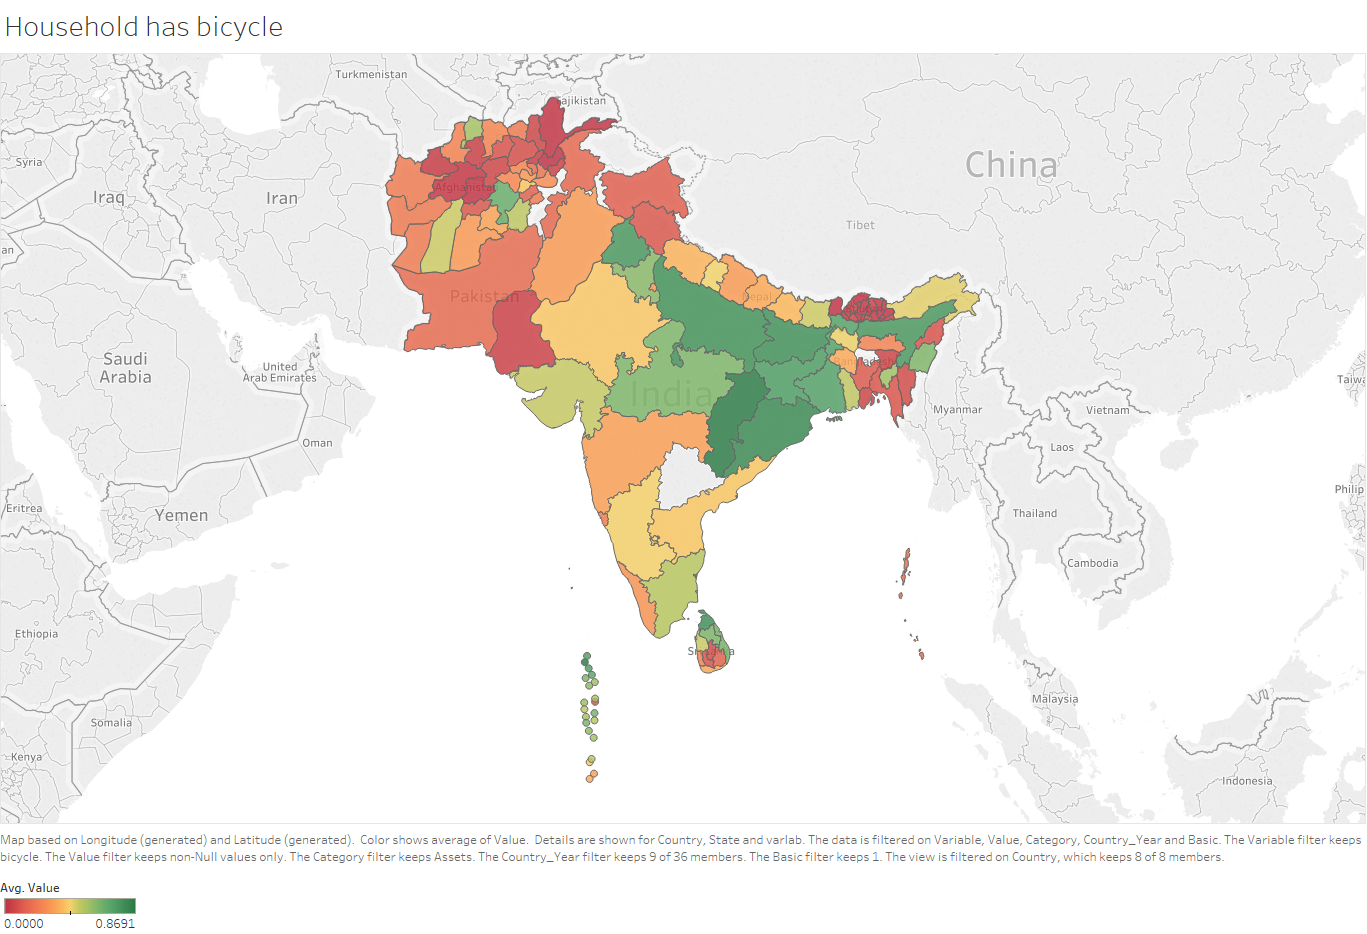
\includegraphics{figures/bicycle.png}}

\chapter*{About the Authors}\label{about-the-authors}
\addcontentsline{toc}{chapter}{About the Authors}

\begin{center}\rule{0.5\linewidth}{\linethickness}\end{center}

The South Asia Region Team for Statistical Development (SARTSD) consists
of:

\begin{itemize}
\item
  Raul Andres Castañeda Aguilar
\item
  Jayne Jungsun Yoo
\item
  Francisco Javier Parada Gomez Urquiza
\end{itemize}

Please let us know if you have any questions and do not hesitate to
share any of your feedback:
\href{mailto:fparadagomezurqu@worldbank.org}{
\includegraphics{figures/mail.png}}

\chapter*{Content}\label{content}
\addcontentsline{toc}{chapter}{Content}

\begin{center}\rule{0.5\linewidth}{\linethickness}\end{center}

\textbf{Part 1} presents the Metadata Analysis, which may be broadly
described as an overview of the household survey questionnaires and
other survey characteristics. This part studies the household surveys'
raw data, sampling methodology, coverage, data capturing methods, and
ability to measure food, non-food, durables, and housing expenditures.

\textbf{Part 2} presents the harmonized variables in the South Asia
Micro Database (SARMD). We inspect the quality of these harmonized
variables and verify that each harmonized variable has been constructed
properly. Two kinds of quality checks of the harmonized data have been
conducted. A static quality check evaluates whether the harmonized
variables are present and whether there is a high percentage of missing
values. It also delves deeper into variables that may be interrelated
with other variables. For example, a high percentage of households that
have access to a television, but do not have access to electricity may
raise questions on how these variables were constructed. A dynamic
quality check evaluates the inconsistencies in measurement of harmonized
data over time. It provides a better overview on whether categorical
variables have changed over time. Changes in poverty and inequality
measures are also analyzed over time.

\textbf{Part 3} presents some examples of how harmonized data in SARMD
may be used for research purposes.

\chapter{Introduction to poverty measures in South
Asia}\label{introduction-to-poverty-measures-in-south-asia}

\begin{center}\rule{0.5\linewidth}{\linethickness}\end{center}

\begin{figure}[htbp]
\centering
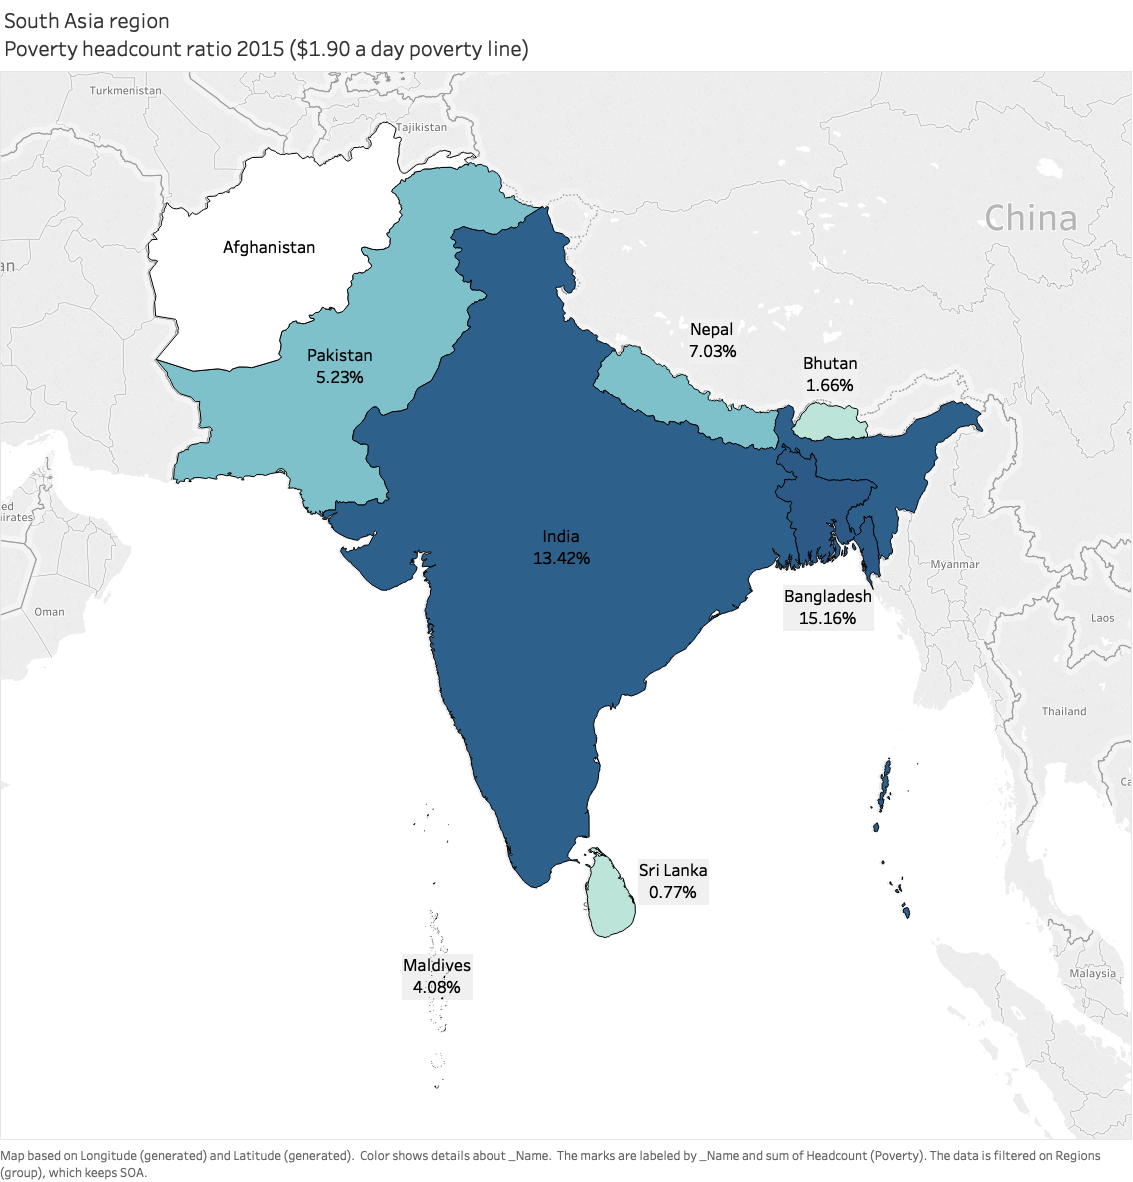
\includegraphics{figures/nice_map.png}
\caption{}
\end{figure}

According to the
\href{http://www.worldbank.org/en/publication/poverty-and-shared-prosperity}{Poverty
and Shared Prosperity Report (2018)}, the number of extreme poor in
South Asia dropped to 216 million people in 2015, compared to half a
billion in 1990, and Nigeria may already have overtaken India as the
country with the most extreme poor in the world. Still, to achieve the
\href{https://www.un.org/sustainabledevelopment/poverty/}{Sustainable
Development Goals}, progress in poverty reduction needs to continue in
India and the rest of South Asia.

The latest poverty measures from the Poverty and Shared Prosperity
Report (2018) are shown in Table \ref{tab:pspr}:

\begin{table}[t]

\caption{\label{tab:pspr}Poverty Measures in Poverty and Shared Prosperity Report (2018)}
\centering
\begin{tabular}{llrrrrr}
\toprule
Country & Survey year(s) & Population & Number of poor (millions) & Poverty rate (\%) & Poverty gap (\%) & Poverty gap/rate (\%)\\
\midrule
India & 2011.5 & 1311.19 & 175.7 & 13.42 & 2.4 & 17.7\\
Bangladesh & 2010 and 2016 & 160.53 & 24.4 & 15.16 & 2.8 & 18.1\\
Pakistan & 2013.5 and 2015.5 & 190.38 & 9.9 & 5.23 & 0.7 & 13.2\\
Nepal & 2010.17 & 28.57 & 2.0 & 7.03 & 1.4 & 19.8\\
Sri Lanka & 2012.5 and 2016 & 25.00 & 0.2 & 0.77 & 0.1 & 11.7\\
\addlinespace
Bhutan & 2012 and 2017 & 0.81 & 0.0 & 1.66 & 0.3 & 16.3\\
Maldives & 2009.5 & 0.37 & 0.0 & 4.08 & 0.8 & 20.3\\
Afghanistan & NA & 35.53 & NA & NA & NA & NA\\
\bottomrule
\end{tabular}
\end{table}

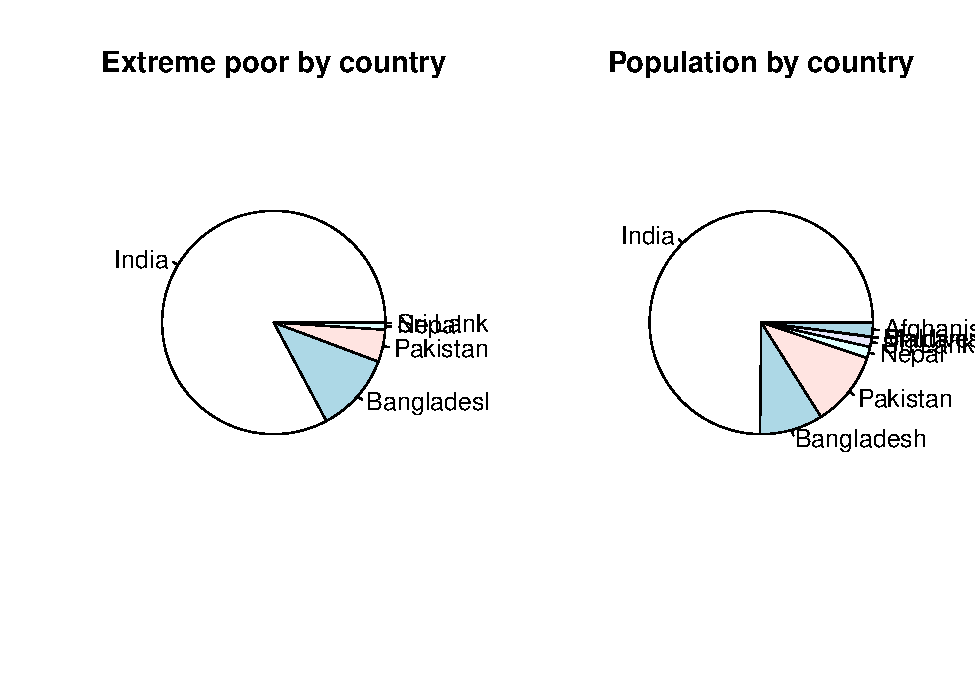
\includegraphics{bookdown-demo_files/figure-latex/pspr-1.pdf}

Based on the
\href{http://www.worldbank.org/en/publication/poverty-and-shared-prosperity}{Poverty
and Shared Prosperity Report (2018)}, we can provide the following
highlights:

\begin{quote}
\begin{itemize}
\tightlist
\item
  In 2015, South Asia accounted for 29\% of the people living in extreme
  poverty worldwide (216 million extreme poor in South Asia out of the
  estimated 736 million extreme poor worldwide).
\item
  Four out of five extreme poor in the South Asia region reside in
  India. Despite a poverty rate of 13.42 percent, India's large
  population of 1.3 billion results in a high absolute number of poor
  (approximately 176 million poor people in 2015).
\item
  Bangladesh has made remarkable progress in reducing poverty, but its
  large population still maintains it in second place within the region
  in terms of absolute number of poor (24.4 million extreme poor in
  2016).
\item
  The third place is Pakistan, which has a larger population than
  Bangladesh, but a smaller amount of extreme poor (9.9 million extreme
  poor in 2015). Pakistan has seen a consistent and significant decline
  in poverty over the 14 years from 2001 to 2015.
\item
  Bhutan and Sri Lanka are considered development success stories where
  extreme poverty has become rare, although a large share of the
  population subsists on slightly more than the extreme poverty line. In
  the Maldives, extreme poverty is nearly nonexistent according to the
  latest survey data.
\end{itemize}
\end{quote}

Even as much of the region leaves extreme poverty behind, poverty is
becoming more entrenched and harder to root out in certain areas,
particularly in countries burdened by violent conflict and weak
institutions. Nepal experienced devastating earthquakes in 2015 and
remains predominantly rural, with the highest share of labor force in
agriculture (73\%) in the region as of 2016. The Maldives were
devastated by the 2004 tsunami while its tourism industry is seriously
threatened by climate change. In the case of Afghanistan, poverty is
increasing as violence continues to affect the security of livelihoods
and economic activity in the country.

The World Bank's poverty measures for South Asia provided by
\href{http://iresearch.worldbank.org/PovcalNet/home.aspx}{PovcalNet} are
described in Table \ref{tab:povcalnet} and may be accessed by
interacting with the following figure:

\href{https://tab.worldbank.org/\#/site/WBG/views/SAR_MNA_Poverty/PovcalNet}{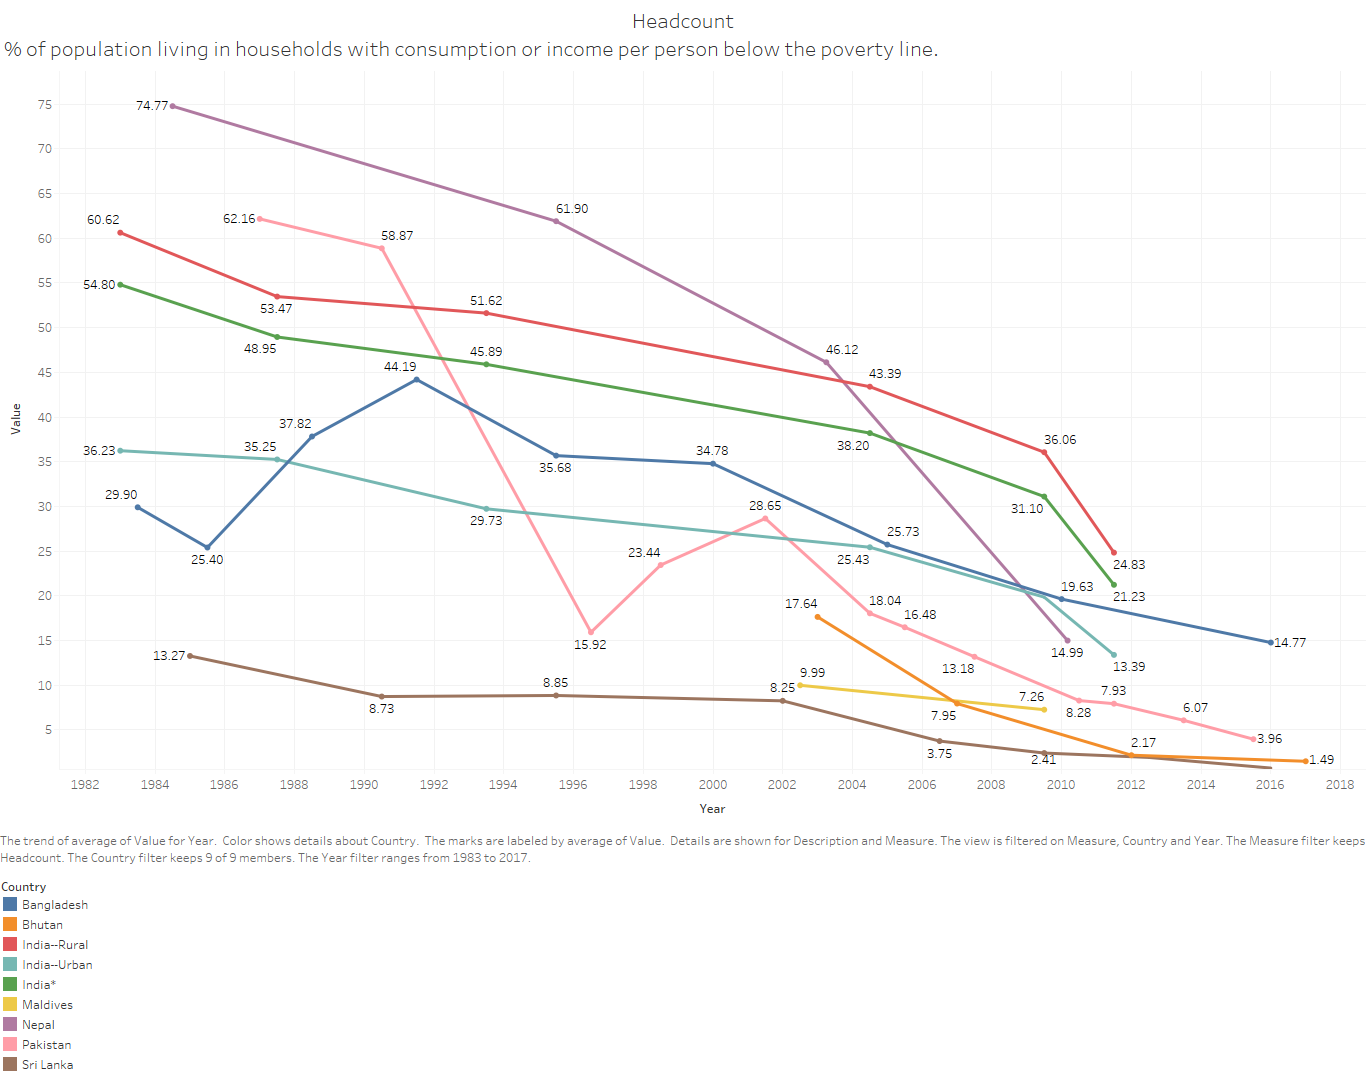
\includegraphics{figures/Povcalnet.png}}

\begin{table}[t]

\caption{\label{tab:povcalnet}Poverty Measures in PovcalNet}
\centering
\begin{tabular}{ll}
\toprule
Measure & Description\\
\midrule
Gini & A measure of inequality between 0 (everyone has the same income) and 100 (richest person has all the income).\\
Headcount & \% of population living in households with consumption per person below the poverty line.\\
Mean & Average monthly household per capita consumption expenditure from the survey in 2011 PPP.\\
Median & Median of monthly household per capita consumption expenditure from the survey in 2011 PPP.\\
MLD & Mean log deviation is an index of inequality, given by the mean across the population of the log of the overall mean divided by individual income.\\
\addlinespace
Population & Country's population in millions.\\
Povgap & The mean shortfall of income from the poverty line. The mean is based on the entire population treating the nonpoor as having a shortfall of zero, and the shortfall is expressed as a proportion of the poverty line.\\
Povline & Poverty line in 2011 PPP per day. The default poverty line is \$1.90 per day.\\
Squared & The mean squared shortfall of income from the poverty line. The mean is based on the entire population treating the nonpoor as having a shortfall of zero, and the shortfall is expressed as a proportion of the poverty line (and then squared).\\
Watts & This is the mean across the population of the proportionate poverty gaps, as measured by the log of the ratio of the poverty line to income, where the mean is formed over the whole population, counting the nonpoor as having a zero poverty gap.\\
\bottomrule
\end{tabular}
\end{table}

\chapter{Poverty measurement
methodology}\label{poverty-measurement-methodology}

\begin{center}\rule{0.5\linewidth}{\linethickness}\end{center}

The World Bank set a target of reducing extreme poverty to less than 3
percent by 2030 and to ensure continued focus and steady progress toward
the goal, the institution set an interim target of 9 percent by 2020.
Progress towards this goal is measured by monitoring the share of the
global population living below the international poverty line, currently
set at US\$1.90 in 2011 purchasing power parity (PPP) dollars. All eight
countries in South Asia measure the international extreme poverty status
of an individual by comparing consumption expenditures per capita
against this poverty line.

This book overviews the data availability of household consumption
surveys in the region of South Asia and their challenges for poverty
measurement. The starting point in monitoring progress in poverty
reduction and enhancing shared prosperity in the region is to have
household consumption survey data that are not only available at
reasonably frequent intervals, but are also comparable over time
(\citet{serajuddin2015data}). Spatial and temporal adjustments are
necessary to take into account differences in costs of living.

First, a consumer price index (CPI) is necessary to measure by how much
the general price level in a country has changed over time. Deflating
all nominal expenditures to real expenditures allows to ensure that
welfare comparisons between two periods are not being driven by
inflation. The following figure displays how the CPI has changed for
each country over time.

\begin{figure}[htbp]
\centering
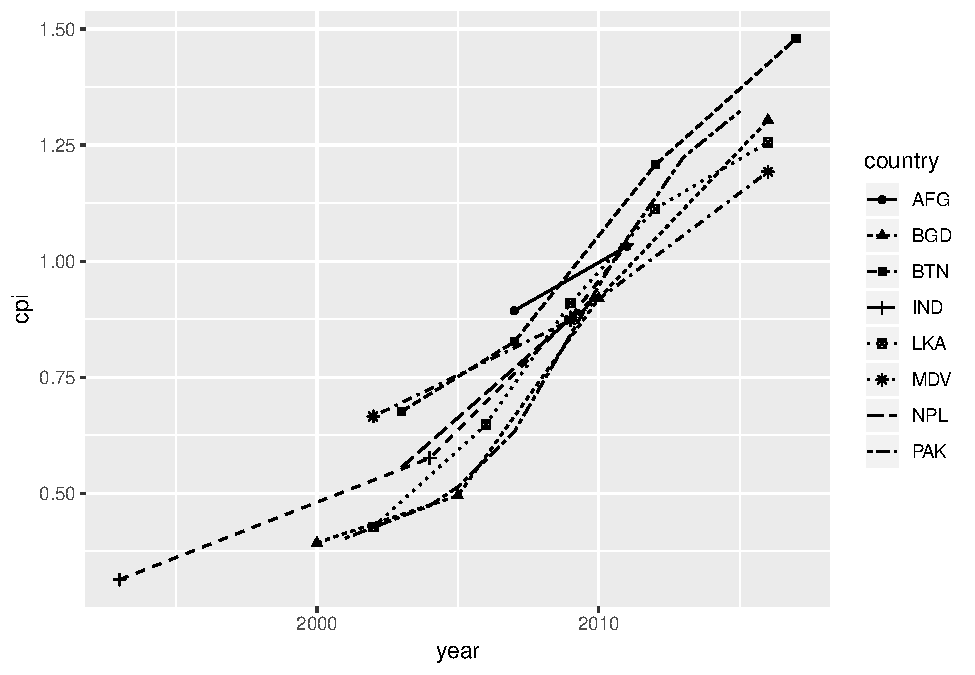
\includegraphics{bookdown-demo_files/figure-latex/cpi-1.pdf}
\caption{\label{fig:cpi}\href{https://tab.worldbank.org/\#/site/WBG/views/SAR_MNA_Summary/LineChart}{Consumer
Price Index (CPI)}}
\end{figure}

Second, spatial price differences, typically between urban and rural
areas, can also be large and it is important to take them into account.
In South Asia, price levels for rural households are often lower than
for urban households. The ideal way to control for spatial differences
in prices is to use a Paasche or Laspeyres index to account for
differences in the cost of living across space.

Third, it is necessary to convert expenditures to a common currency
taking into account purchasing power. At present, data on purchasing
power parity (PPP) comes from the International Comparison Program (ICP)
collected in 2011, which is absent for Afghanistan. Purchasing power
parities (PPPs) are the rates of currency conversion that equalize the
purchasing power of different currencies by eliminating the differences
in price levels between countries. In their simplest form, PPPs show the
ratio of prices in national currencies of the same good or service in
different countries. PPPs are also calculated for groups of products and
for each of the various levels of aggregation up to and including GDP.
The basket of goods and services priced is a sample of all those that
are a part of final expenditure: household consumption, government
services, capital formation and net exports, covered by GDP. This
indicator is measured in terms of national currency per US dollar.

\begin{longtable}[]{@{}ccc@{}}
\toprule
Country & Currency & ICP 2011\tabularnewline
\midrule
\endhead
Afghanistan & Afghan afghani & NA\tabularnewline
Bangladesh & Bangladeshi taka & 24.8493\tabularnewline
Bhutan & Bhutanese ngultrum & 16.96292\tabularnewline
India & Indian rupee & 13.98707\tabularnewline
Maldives & Maldivian rufiyaa & 10.67606\tabularnewline
Nepal & Nepalese rupee & 25.75928\tabularnewline
Pakistan & Pakistani rupee & 25.41426\tabularnewline
Sri Lanka & Sri Lankan rupee & 42.21894\tabularnewline
\bottomrule
\end{longtable}

A fourth adjustment is dividing total household expenditure by some
measure of the number of people in the household, and to assign the
resulting per capita welfare measure to each household member as an
individual. Later in the applications, we show how larger households
typically have lower per capita expenditure levels than smaller
households. In South Asia, the consequences of dividing total household
expenditures by a greater number of individuals would not be complete
without considering the extent of economies of scale within the
household and a discussion of how much children and the elderly
typically consume compared to adults.

A headcount ratio may be calculated as in the STATA example below.

\begin{Shaded}
\begin{Highlighting}[]
\NormalTok{**STATA Example**}

\FunctionTok{# Calculating poverty headcounts with 1.90 poverty line}
\NormalTok{gen welfare=total_exp/hsize}
\NormalTok{welf_ppp = welfare/cpi2011/icp2011/365}
\NormalTok{gen poor190 = wefl_ppp < 1.90}
\NormalTok{sum poor190 [aw=wgt]}
\end{Highlighting}
\end{Shaded}

The FGT measures devised by Foster, Greer and Thorbecke (1984) remain
the most commonly used to measure poverty. They are defined as:

\[\begin{equation}
P_{\alpha}=\frac{1}{N}\sum^{N}_{i=1}I_{i}\left(\frac{\bar{u}-u_{i}}{\bar{u}}\right)^{\alpha}
\end{equation}\]

where N is the sample size, \[\bar{u}\] is the scalar-valued poverty
line, \[u_{i}\] is the flow-based measure of welfare (income,
expenditures, assets), \[I_{i}\] is an indicator variable taking value
one if \(u_{i} < \bar{u}\) and zero otherwise, and \[\alpha\] is a
parameter reflecting the weight placed on the severity of poverty.
Setting \[\alpha =0\] yields the poverty headcount ratio \(P_{0}\) (the
share of a population falling below the poverty line). The higher order
measures, \[P_{1}\] and \[P_{2}\], yield the poverty gap measure (the
money metric measure of the average financial transfer needed to bring
all poor households up to the poverty line) and the squared poverty gap
(an indicator of the severity of poverty that is sensitive to the
distribution of well-being among the poor). As we progress from
\[P_{0}\] to \[P_{1}\] to \[P_{2}\], the \[P_{\alpha}\] measure gets
more and more sensitive to extremely low incomes.

\part{Metadata Analysis}\label{part-metadata-analysis}

\chapter{Metadata Analysis}\label{metadata}

\begin{center}\rule{0.5\linewidth}{\linethickness}\end{center}

\href{https://tab.worldbank.org/\#/site/WBG/views/SAR_MNA_Summary/Cover}{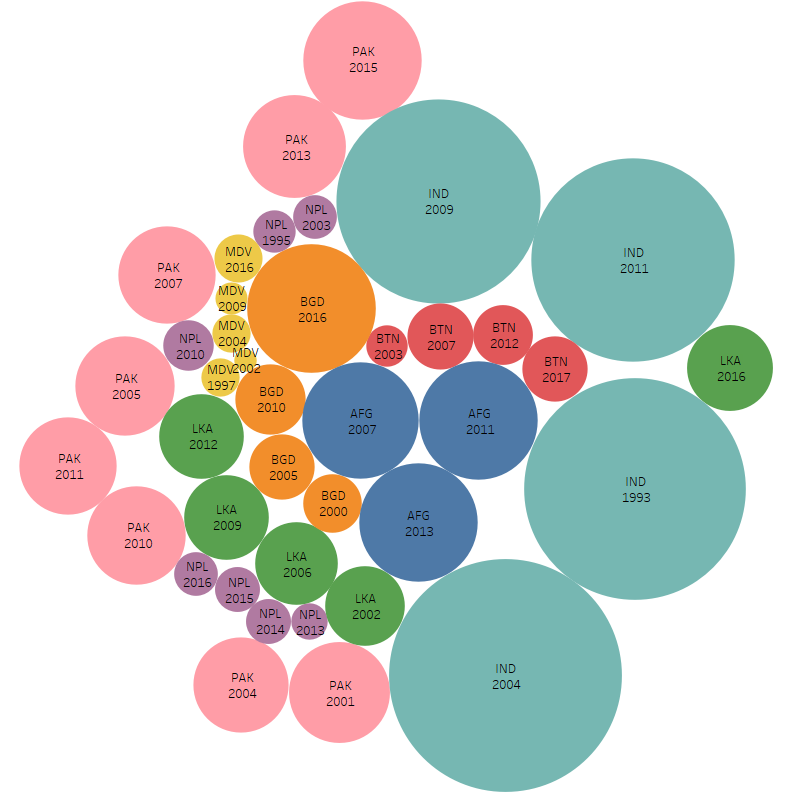
\includegraphics{figures/Bubbles.png}}

This chapter provides an overview of household surveys metadata in the
South Asia Micro Database (SARMD) with the support of a series of
accompanying Tableau dynamic dashboards. You may access the Tableau
dashboards by clicking on them and on the figures' titles. SARMD is a
regional database of socio-economic indicators established in 2014 and
managed by the South Asia Region Team for Statistical Development
(SARTSD). It follows the Global Monitoring Database (GMD) harmonization
guidelines, including the construction of the welfare aggregate used for
global poverty monitoring. SARMD consists of raw household survey data,
documentation, questionnaires, and a repository of do files to
reconstruct harmonized variables, consumption aggregates, and poverty
estimates. SARMD currently includes the eight countries in the region
(Afghanistan, Bangladesh, Bhutan, India, Maldives, Nepal, Pakistan, and
Sri Lanka), contemplates forty-three surveys, and contains close to a
hundred harmonized variables covering the 1993-2017 period. Table
\ref{tab:latest} shows the latest available household surveys in SARMD
and provides links to the National Statistics Offices' websites.

\begin{table}[t]

\caption{\label{tab:latest}Latest household surveys available in SARMD}
\centering
\begin{tabular}{lllr}
\toprule
Country & Name of the survey & National Statistics Office & Sample size: Number of households\\
\midrule
Afghanistan, 2016 & Living Conditions Survey & [Central Statistics Organization](http://cso.gov.af/) & NA\\
Bangladesh, 2016 & Household Income and Expenditure Survey & [Bangladesh Bureau of Statistics](http://bbs.gov.bd/) & 46068\\
Bhutan, 2017 & Living Standards Survey & [National Statistics Bureau](http://nsb.gov.bt) & 11396\\
India, 2017 & National Sample Survey & [Ministry of Statistics and Programme Implementation ](http://mospi.gov.in/) & NA\\
Maldives, 2016 & Household Income and Expenditure Survey & [National Bureau of Statistics](http://statisticsmaldives.gov.mv/) & 4910\\
\addlinespace
Nepal, 2016 & Annual Household Survey & [Central Bureau of Statistics](http://cbs.gov.np/) & 4500\\
Pakistan, 2015 & Social and Living Standards Measurement Survey & [Pakistan Bureau of Statistics](http://www.pbs.gov.pk/) & 24238\\
Sri Lanka, 2016 & Household Income and Expenditure Survey & [Department of Census and Statistics](http://www.statistics.gov.lk/) & 21756\\
\bottomrule
\end{tabular}
\end{table}

\section{Inventory}\label{inventory}

Considering that the South Asia region has the second largest poor
population in the world, it is essential to improve the frequency and
regularity of poverty data. Figure \ref{fig:inv} presents the surveys
that make part of the South Asia Micro Database (SARMD). Six countries
have released recent rounds of household surveys (Pakistan 2015,
Afghanistan 2016, Bangladesh 2016, Maldives 2016, Sri Lanka 2016, and
Bhutan 2017) while others are about to release a new round in the next
year (India 2017). Nepal has collected five rounds of its Annual
Household Survey (AHS) while it waits for the fourth round of the Nepal
Living Standards Survey.

Extreme data deprivation may be measured as having less than two data
points in a ten-year period. The inventory section shows that in 2019
the region of South Asia is not considered extremely data deprived.
Still, unless they collect surveys more frequently, three countries are
vulnerable to extreme data deprivation by 2022: Bangladesh, Maldives and
India.

\begin{figure}

{\centering 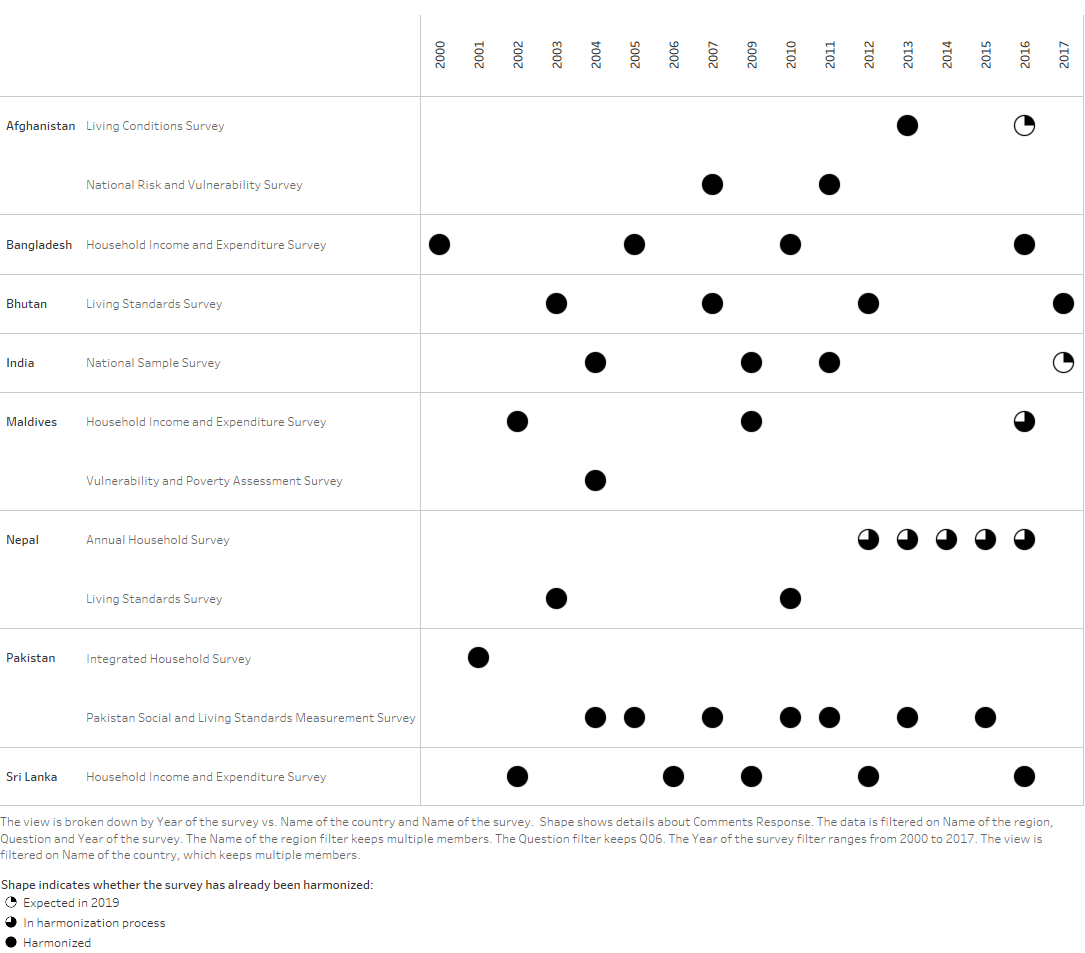
\includegraphics[width=15.07in]{figures/Inventory} 

}

\caption{[SARMD Inventory](https://tab.worldbank.org/#/site/WBG/views/SAR_MNA_Metadata/Availability)}\label{fig:inv}
\end{figure}

\href{https://tab.worldbank.org/\#/site/WBG/views/SAR_MNA_Metadata/Map}{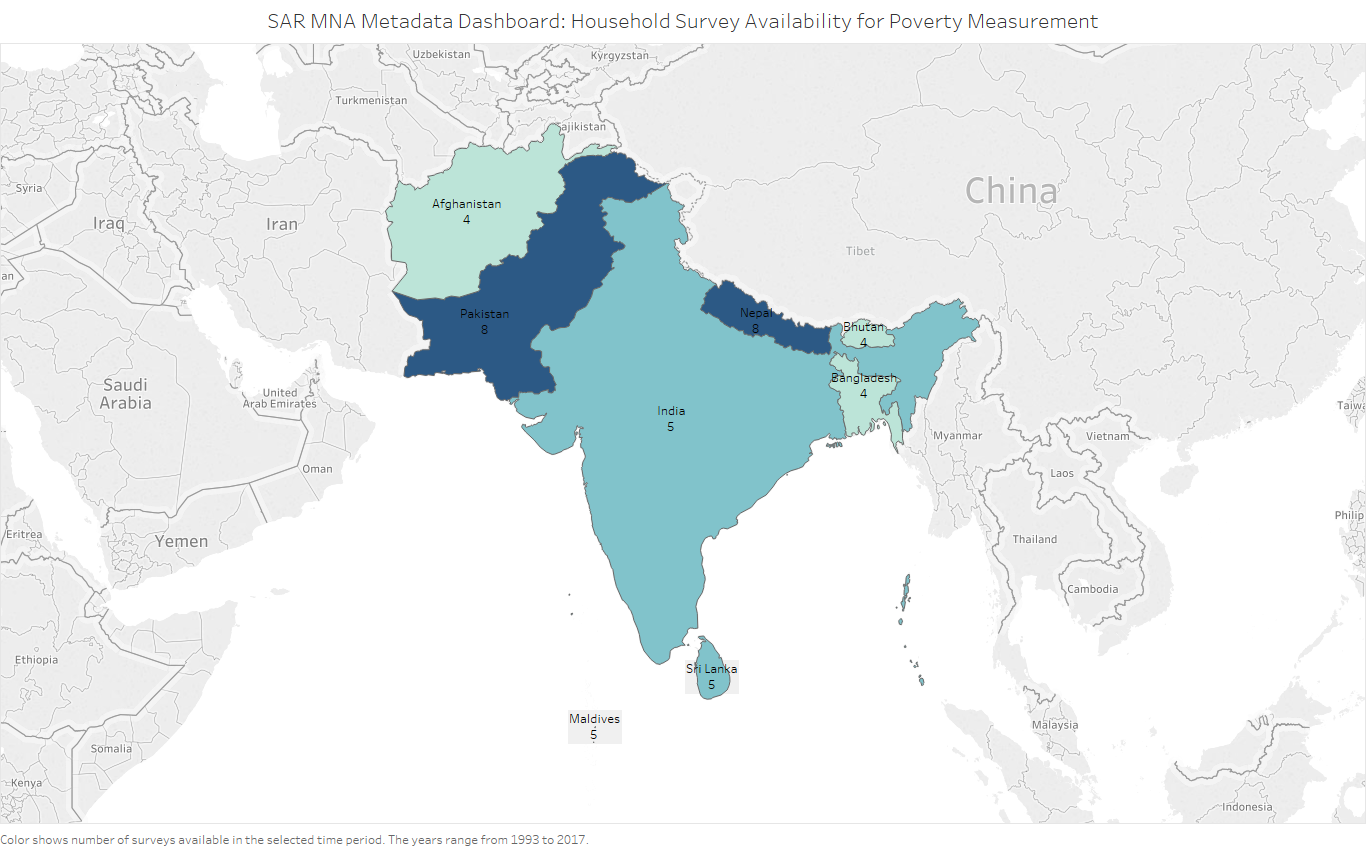
\includegraphics{figures/Inventory_map.png}}

\section{Sample size}\label{sample-size}

India's household survey is by far the largest covering 100,000
households in the 2009 and 2011 rounds as shown in Figure
\ref{fig:ssize}. Maldives' survey is the smallest covering 4,910
households in the 2016 round. Most surveys have a stable sample size
over time. A clear exception is Bangladesh 2016, which almost quadrupled
its sample size compared to its predecessor in 2010. Household size is
close to seven in Afghanistan and Pakistan, and much closer to 4-5 in
the rest of the countries. Sri Lanka is the country with the smallest
average household size. All surveys cover both urban and rural areas and
the proportion of rural surveys can vary significantly. The latest
Afghanistan and Sri Lanka surveys have collected a large proportion of
surveys in rural households (above 80\% of households).

\begin{figure}

{\centering 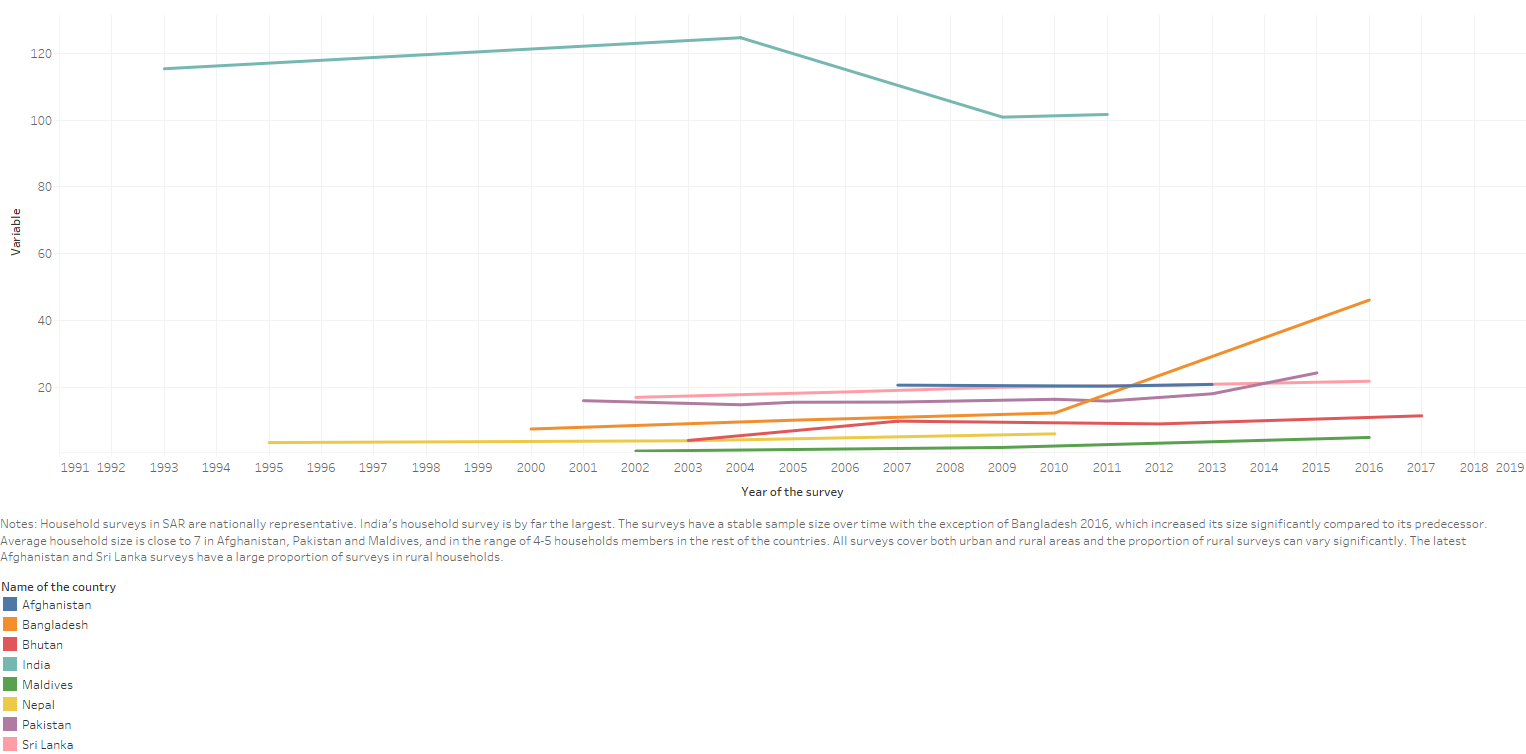
\includegraphics[width=21.19in]{figures/Survey_size} 

}

\caption{[Sample Size](https://tab.worldbank.org/#/site/WBG/views/SAR_MNA_Metadata/Lines)}\label{fig:ssize}
\end{figure}

\section{Household survey description by
country}\label{household-survey-description-by-country}

The content of these surveys varies widely and their comparison over
time even within the same country is a major challenge. We provide a
brief overview of survey collection for each country below:

\subsection{Afghanistan}\label{afghanistan}

\begin{flushleft}
\includegraphics[width=0.4\linewidth]{figures/Flag_of_Afghanistan} \end{flushleft}

The Afghanistan Living Conditions Survey (ALCS) 2016-2017 represents the
entire population of Afghanistan and may be disaggregated by urban and
rural population, and by the nomadic Kuchi population. Previously, the
survey was named National Risk and Vulnerability Assessment (NRVA). This
survey covers 35 strata, 34 for the provinces of Afghanistan and one for
the nomadic Kuchi population. Stratification by season was achieved by
equal distribution of data collection over 12 months within the
provinces for the latest round between April 2016 and March 2017. In the
first three months of fieldwork, areas that were inaccessible due to
insecurity were replaced by sampled areas that were scheduled for a
later month, in the hope that over time security conditions would
improve. Eventually, some clusters in inaccessible areas were replaced
by clusters that excluded insecure areas.

The Central Statistics Organization (CSO) (\url{http://cso.gov.af/}) has
used the ALCS 2016 to report that poverty rates in Afghanistan have
experienced a sharp increase since 2011-12, especially in rural areas.
Households of larger size face a higher poverty rate. Although larger
land size is no guarantee for escaping poverty, the smaller the size of
land owned by households, the higher is the proportion that falls below
the poverty line. Lack of education is another important correlate of
poverty in Afghanistan. Low levels of educational attainment are
pervasive and households with illiterate heads account for 74 percent of
the population.

\subsection{Bangladesh}\label{bangladesh}

\begin{flushleft}
\includegraphics[width=0.4\linewidth]{figures/Flag_of_Bangladesh} \end{flushleft}

The Household Income and Expenditure Survey (HIES) is the comprehensive
nationally representative survey used to measure poverty in Bangladesh.
The HIES 2016/17 is the fourth round in the series of HIES conducted by
the Bangladesh Bureau of Statistics (BBS) (\url{http://bbs.gov.bd/}) in
2000, 2005, and 2010. As of 2016, Bangladesh had eight administrative
divisions. These were Barisal, Chittagong, Dhaka, Khulna, Mymensingh,
Rajshahi, Rangpur and Sylhet. These 8 divisions of the country were
stratified by rural, urban and city corporation, however, city
corporations were only considered for Dhaka, Chittagong, Khulna and
Rajshahi. This brought the number of strata to 20 (8 rural divisions, 8
urban divisions, and 4 city corporations).

Based on the HIES 2016, the BBS reports that poverty was reduced
substantially between 2010 and 2016. In 2010, the poverty headcount
ratio, using a higher poverty line, was 31.5\% which reduced to 24.3\%
in 2016. Using a lower poverty line the headcount ratio also reduced
from 17.6\% in 2010 to 12.9\% in 2016. Using the higher upper poverty
line, Rangpur had the highest incidence of poverty at 47.2\%, followed
by Mymensingh 32.8\%, Rajshahi 28.9\% and Khulna 27.5\%. On the other
hand, Dhaka recorded the lowest headcount ratio of 16.0\%, followed by
Sylhet 16.2\%, and Chittagong 18.4\%.

\subsection{Bhutan}\label{bhutan}

\begin{flushleft}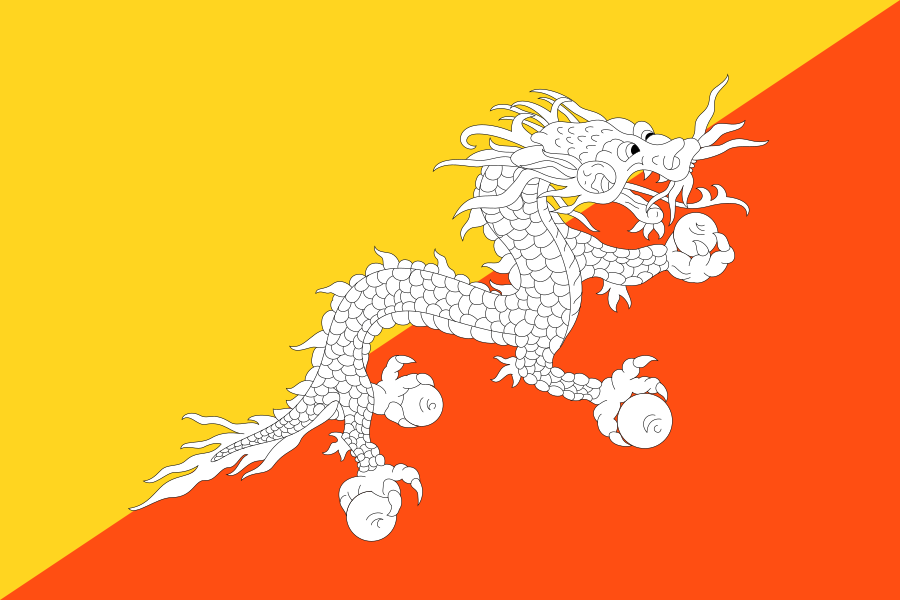
\includegraphics[width=0.4\linewidth]{figures/Flag_of_Bhutan} \end{flushleft}

The Bhutan Living Standards Survey (BLSS) 2017 is the fourth in a series
of living standards surveys undertaken by the National Statistics Bureau
(NSB) (\url{http://nsb.gov.bt}). Earlier surveys were done in 2003,
2007, and 2012 to collect information on the demographics, education,
health, employment, housing, access to services, asset ownership,
credit, self-perceived poverty, and happiness of the population. The
BLSS 2017 included 11,660 households with 48,639 individuals. The sample
for BLSS 2017 was designed to provide estimates for many indicators on
the living conditions of Bhutanese in both urban and rural areas of the
twenty Dzongkhags, including the four Thromdes (Thimphu, Phuentsholing,
Gelephu and Samdrup Jongkhar).

The NSB reports a population poverty rate of 8.2\% in 2017. The 2017
BLSS shows that the mean monthly household expenditure for the country
is Nu33,542: Nu45,508 in urban areas, and Nu26,937 in rural areas. The
mean monthly per capita household expenditure is Nu7,939. The monthly
per capita household expenditure ofNu11,452 in urban areas is 85\%
higher than that in rural areas (Nu6,174). The mean per capita
expenditure of households in the richest per capita consumption quintile
of Nu17,802 is more than seven times that of households in the poorest
per capita consumption quintile (Nu2,468).

The NSB has also analyzed subjective happiness ratings by dzongkhags.
Pema Gatshel is the happiest Dzongkhag (94\%) followed by Samtse (more
than 88\%) and Trongsa Dzongkhags (more than 86\%). The exception is
Dagana Dzongkhag, where only four in every 10 respondents reported they
are happy. Dagana also stands out as the Dzongkhag with the highest
poverty rate.

\subsection{India}\label{india}

\begin{flushleft}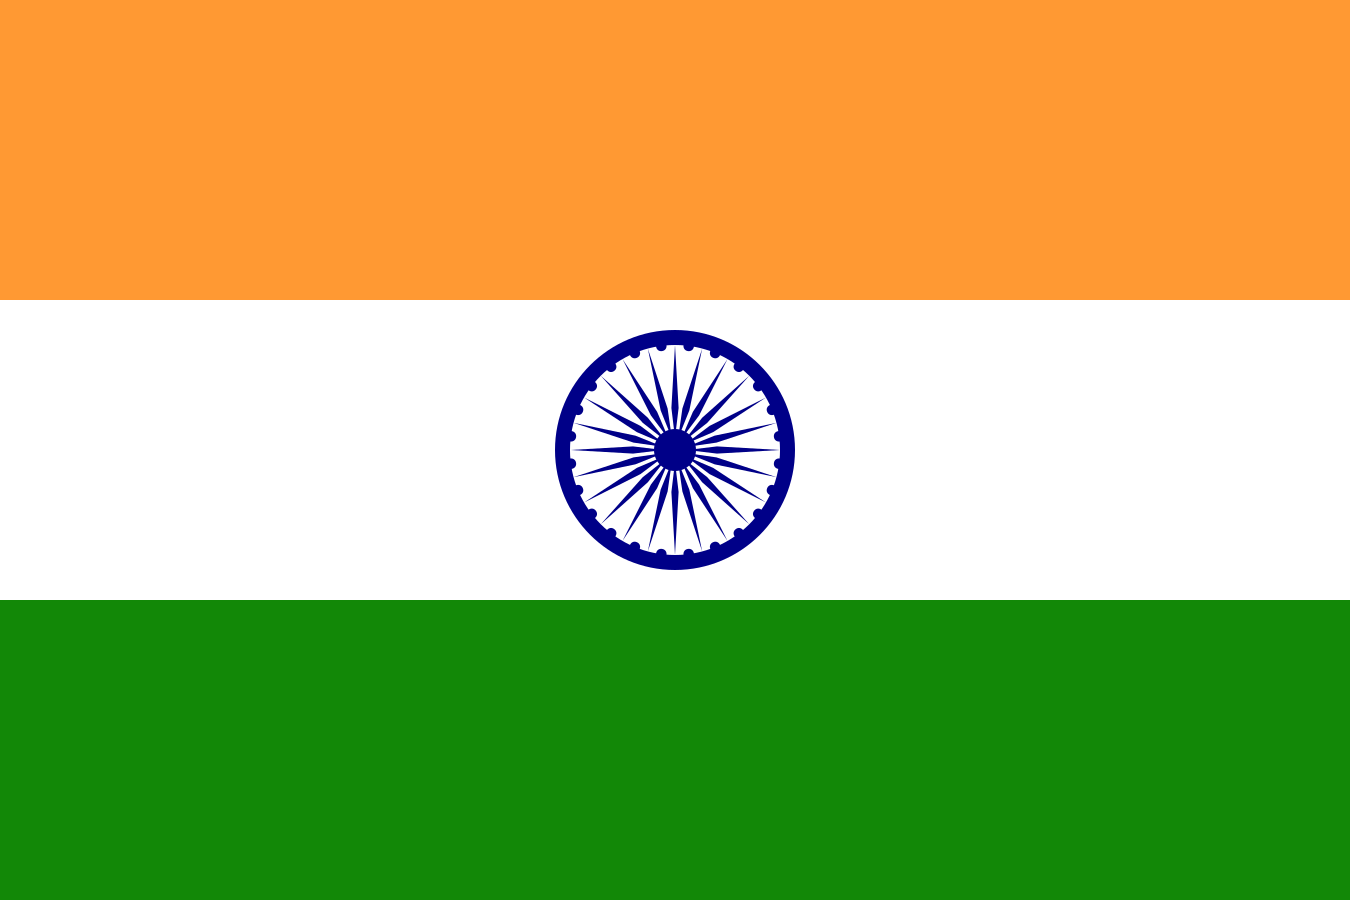
\includegraphics[width=0.4\linewidth]{figures/Flag_of_India} \end{flushleft}

Despite India's remarkable progress in reducing poverty, poverty remains
widespread especially in the highly-populated Eastern states of Bihar,
Chhattisgarh, Jharkhand, Madhya Pradesh, Odisha, and Uttar Pradesh. The
national poverty estimates for India are based on rounds of Household
Consumption Expenditure Surveys conducted by the National Sample Survey
Office (NSSO) (\url{http://mospi.gov.in/}). The 68th round (July
2011-June 2012) of NSS is designated to measure household consumer
expenditure, employment, and unemployment. The 68th round is the most
recent round for which consumption data is currently available in SARMD.
The survey covers the whole of the Indian Union except interior villages
of Nagaland situated beyond five kilometers of the bus route and
villages in Andaman and Nicobar Islands which remain inaccessible
throughout the year.

In the 68th round two schedule types exist. The two schedule types
differ by their reference periods (in the 68th round, Schedule Type 1
and Schedule Type 2 use the same reference periods as in the 66th
round). Sample households were divided into two sets: Schedule Type 1
was canvassed in one set and Schedule Type 2 in the other. Schedule Type
1 requires that for certain non-food items (clothing, bedding, footwear,
education, medical (institutional), durable goods), the same household
should report data for two reference periods: the last 30 days and the
last 365 days. For these same non-food items, the reference period used
in Schedule Type 2 is only the last 365 days. As in the 66th round,
items of food, pan, tobacco and intoxicants (food-plus category) are
split into 2 blocks, block 5.1 and block 5.2, instead of being placed in
a single block. Block 5.1 consists of cereals, pulses, milk and milk
products, sugar and salt. This block has a reference period of 30 days
in both Schedule Type 1 and Schedule Type 2. Block 5.2 consists of the
other items of food, along with pan, tobacco and intoxicants. This block
is assigned a reference period of last 30 days in Schedule Type 1 and a
reference period of last 7 days in Schedule Type 2.

\subsection{Maldives}\label{maldives}

\begin{flushleft}
\includegraphics[width=0.4\linewidth]{figures/Flag_of_Maldives} \end{flushleft}

The latest round of the Maldives Household Income and Expenditure Survey
(HIES) took place in 2016 with other rounds conducted in 2003 and
2009-10. The sample (4,910 households and 26,453 individuals) was
designed by the National Bureau of Statistics (NBS)
(\url{http://statisticsmaldives.gov.mv/}) in such a way that the results
are representative for each of the 20 individual atolls and the capital
Male'. The HIES 2016 questionnaire was completely revised and includes
important survey improvements, particularly in the measurement of
poverty, which also hinders comparability with past survey years
(\citet{maldives_2018}). Improvements include the inclusion of rent and
durable goods in the construction of the welfare aggregate, and change
from diary to recall of food items. According to the national poverty
line, the poverty is highest in Gdh. atoll and the lowest is in V.
atoll. The Gini coefficient for Maldives is 0.313, and is slightly
higher in Male' than in the Atolls.

\subsection{Nepal}\label{nepal}

\begin{flushleft}
\includegraphics[width=0.35\linewidth]{figures/Flag_of_Nepal.svg} \end{flushleft}

National poverty estimates in Nepal are produced by the Central Bureau
of Statistics (CBS) (\url{http://cbs.gov.np/}). The last national
poverty update in Nepal was based on the 2010 Nepal Living Standard
Survey (NLSS-III). Three rounds of the Nepal Living Standards Surveys
(NLSS) have been carried out in 1995/96, 2003/04, and 2010/11. These
surveys follow the World Bank's Living Standards Measurement Survey
methodology and cover a wide range of topics: demography, consumption,
income, access to facilities, housing, education, health, employment,
credit, remittances, etc. While the data from the next round of the NLSS
is unlikely to be available until the end of 2019, the CBS has conducted
five rounds of the Annual Household Survey (AHS) from 2012-13 to
2016-17. Before the release of the next national poverty rate estimates
from NLSS-IV, the World Bank plans to prepare the poverty update report
using the recent AHS.

The new administrative division of Nepal consists of seven provinces,
some of which have not been named yet. These seven provinces are
currently referred as Province No. 1, Province No. 2, Province No. 3,
Gandaki, Province No. 5, Karnali, and Sudurpashchim. This new
administrative division of Nepal was implemented with the new
constitution on September 20, 2015. Before 2015, instead of provinces,
Nepal was divided into developmental regions and administrative zones.

\subsection{Pakistan}\label{pakistan}

\begin{flushleft}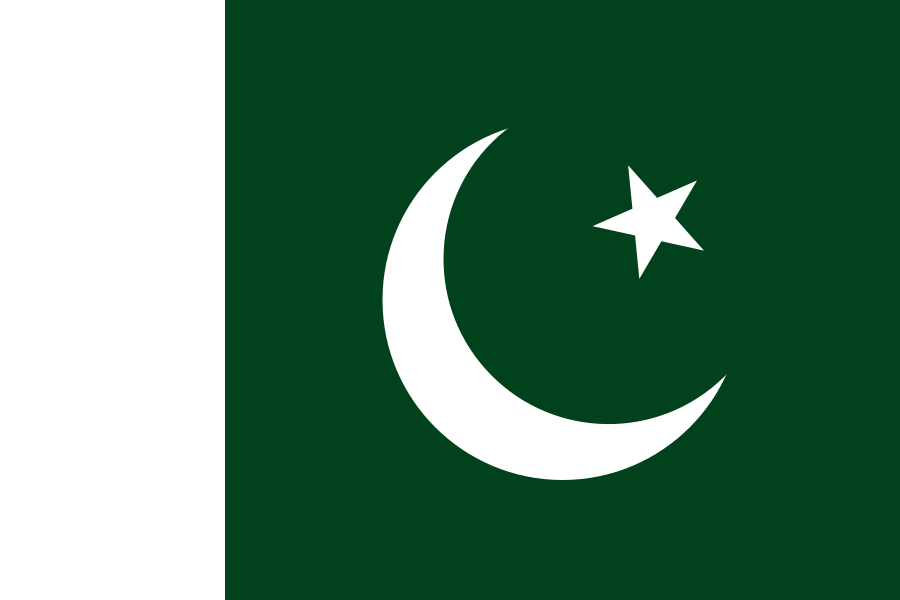
\includegraphics[width=0.4\linewidth]{figures/Flag_of_Pakistan} \end{flushleft}

The latest round of the Pakistan Social and Living Standards Measurement
Survey (PSLM) 2015-2016 conducted by the Pakistan Bureau of Statistics
(PBS) (\url{http://www.pbs.gov.pk/}) covers 24,238 households. It
provides information on household income, savings, liabilities,
consumption expenditures, and consumption patterns at national and
provincial levels. Before this survey, six rounds were conducted during
2004-05, 2005-06, 2007-08, 2010-11, 2011-12 and 2013-14. The PSLM covers
all urban and rural areas of the four provinces of Pakistan (Punjab,
Khyber Pakhtunkhwa, Sindh, and Balochistan) excluding Federally
Administered Tribal Areas (FATA) and military restricted areas.

The incidence of poverty is uneven across Pakistan's provinces. Khyber
Pakhtunkhwa is the province with the lowest poverty headcount in 2015,
while Balochistan accounts for the highest poverty rate. As in the rest
of the region, poverty is higher in rural areas than in urban areas.

\subsection{Sri Lanka}\label{sri-lanka}

\begin{flushleft}
\includegraphics[width=0.4\linewidth]{figures/Flag_of_Sri_Lanka} \end{flushleft}

The Household Income and Expenditure Survey (HIES) conducted by the
Department of Census and Statistics (DCS)
(\url{http://www.statistics.gov.lk/}) is the main data source used to
calculate poverty indices for Sri Lanka. The HIES 2016 is the ninth in
the HIES series and was conducted in January-December 2016. SARMD also
contains four of the previous rounds conducted in 2002, 2006, 2009, and
2012. THE HIES covers all 9 provinces (Central Province, Eastern
Province, North Central Province, Northern Province, North Western
Province, Sabaragamuwa, Southern Province, Uva, and Western Province)
and 25 districts in the country. The survey provides information on
household income and consumption expenditure to measure changes in
living conditions. According to the DCS, the poverty headcount ratio
declined from 6.7\% in 2012/13 to 4.1\% in 2016. Despite progress,
pockets of deep poverty remain in the North and the East. Among the
districts, Kilinochchi district reported the highest headcount index
(18.2\%) and Colombo had the lowest (0.9\%).

\section{Expenditure components}\label{expenditure-components}

We consider four main components for a nominal consumption aggregate:

\subsection{Food}\label{food}

The first component is food expenditures, which should include not only
food produced and/or consumed at home, but also food purchases outside
of home, and food transfers to and from the household. This component is
sometimes thought to be easier to measure than non-food items. When
household members eat from a common pot, it is common to find a single
well-informed individual who can act as respondent and provide
information about how much the household has consumed. Surveys sometimes
include a household food expenditure diary, but this is not common in
South Asia where most information on food is collected based on
recalling what a household has consumed and purchased over the last
seven days.

The ideal reference period should be a week, but in this analysis we
have found reference periods still vary from yearly, to monthly, to
biweekly, to daily across surveys. In recent years, the Indian National
Sample Survey Organization has experimented with 7-day and 30-day recall
periods for a number of items, and discovered that the 7-day recall cuts
Indian poverty rates by half, removing some 200 million people from
dollar-a-day poverty. This is an issue that has not been much
investigated, but has recently moved into the forefront of research. In
other words, methods matter and it is important to standardize data
collection as much as possible.

In most cases, countries modify their food baskets and change their data
collection methods over time. A wide mixture of data collection methods
characterizes the most recent rounds of household surveys. Bangladesh
HIES 2016 collects daily household food consumption (both quantity and
value) for a period of 14 days. In addition, it collects weekly
consumption of a series of spices. Bhutan LSS 2017 collects food
consumption (both quantity and value) by asking the respondent to recall
their consumption in the last seven days, the last thirty days, and the
last year. In some cases, such as Afghanistan LCS 2016, the female
respondents are the ones asked about household food consumption. These
methods can be very diverse and we provide a brief description for the
latest survey available for each country in Table \ref{tab:food}.

\begin{table}[t]

\caption{\label{tab:food}Mixture of collection methods for food at home}
\centering
\begin{tabular}{lrll}
\toprule
Country, Year & Number of food items & Collection method & Quantity and/or Value\\
\midrule
Afghanistan, 2016 & 92 & Recall (weekly) & Quantity\\
Bangladesh, 2016 & 151 & Diary (daily) & Both\\
Bhutan, 2017 & 115 & Recall (weekly, monthly, yearly) & Both\\
India, 2011 & 134 & Recall (multiple) & Both\\
Maldives, 2016 & 146 & Recall (weekly) & Both\\
\addlinespace
Nepal, 2015 & 97 & Recall (weekly) & Both\\
Pakistan, 2015 & 170 & Recal (biweekly) & Both\\
Sri Lanka, 2016 & 198 & Recall (weekly) & Both\\
\bottomrule
\end{tabular}
\end{table}

Food is composed of all edible goods that are purchased and consumed by
the household with the purpose of nourishing. Food baskets are usually
organized by categories into:

\begin{enumerate}
\def\labelenumi{\arabic{enumi}.}
\tightlist
\item
  Cereals and cereal products;
\item
  Meat;
\item
  Fish and other seafood;
\item
  Milk, other dairy products and eggs;
\item
  Oils and fats;
\item
  Fruit and nuts;
\item
  Vegetables, tubers, plantains, cooking bananas and pulses;
\item
  Sugar, confectionery and desserts;
\item
  Salt, sauces and condiments, spices and culinary herbs and seeds.
\end{enumerate}

Alcohol and tobacco are considered non-food items for measuring
purposes, but it is common to find them in the food section of a
questionnaire. In most surveys, households report both quantities and
expenditures for most of the foods they purchase (e.g.~three kilograms
of rice for 5 rupees). However, this is not the norm. For example, the
Afghanistan LCS 2016 asks what was the amount of 92 items used in the
last seven days, but the price of each item is collected separately
through a market price survey.

Besides food produced and consumed at home, the food component should
include food consumed outside the home, both formally such as at
restaurants and cafés, and informally, such as small snacks and drinks.
This component is usually recorded separately and is more likely to
suffer from measurement error. An agreement on how these expenditures
should be recorded has not been reached. For example, Afghanistan LCS
2016 asks for the total amount spent on food and drinks outside of home
in the last month. In contrast, Bhutan LSS 2017 asks how many times did
the household consume food for breakfast, lunch, dinner, snack, etc.
outside of home in the last 7 days and what was the average value of the
purchase.

Another component that is prone to measurement error is food transfers,
which are currently measured unevenly with different collection methods.
We have found that it is more common to find questions regarding
transfers to the household than transfers from the household to other
households. For example, Bhutan LSS 2017 asks what is the total value of
a food item that was received as gift over the past 12 months. However,
it does not ask what amount of the food item has the household
transferred to others.

We provide a
\href{https://tab.worldbank.org/\#/site/WBG/views/SAR_MNA_Metadata/Food}{Tableau
dashboard} where the user may compare surveys according to:

\begin{itemize}
\tightlist
\item
  The number of
  \href{https://tab.worldbank.org/\#/site/WBG/views/SAR_MNA_Metadata/Items}{food
  items} in the food basket
\item
  Whether they collect the quantity and/or value of food consumed at
  home and outside of home
\item
  Data collection methods (diary vs.~recall) as well as their reference
  periods (daily, weekly, bi-weekly, monthly, and/or yearly)
\item
  Information on self-production
\item
  Information on transfers to and from the household
\end{itemize}

\href{https://tab.worldbank.org/\#/site/WBG/views/SAR_MNA_Metadata/Food}{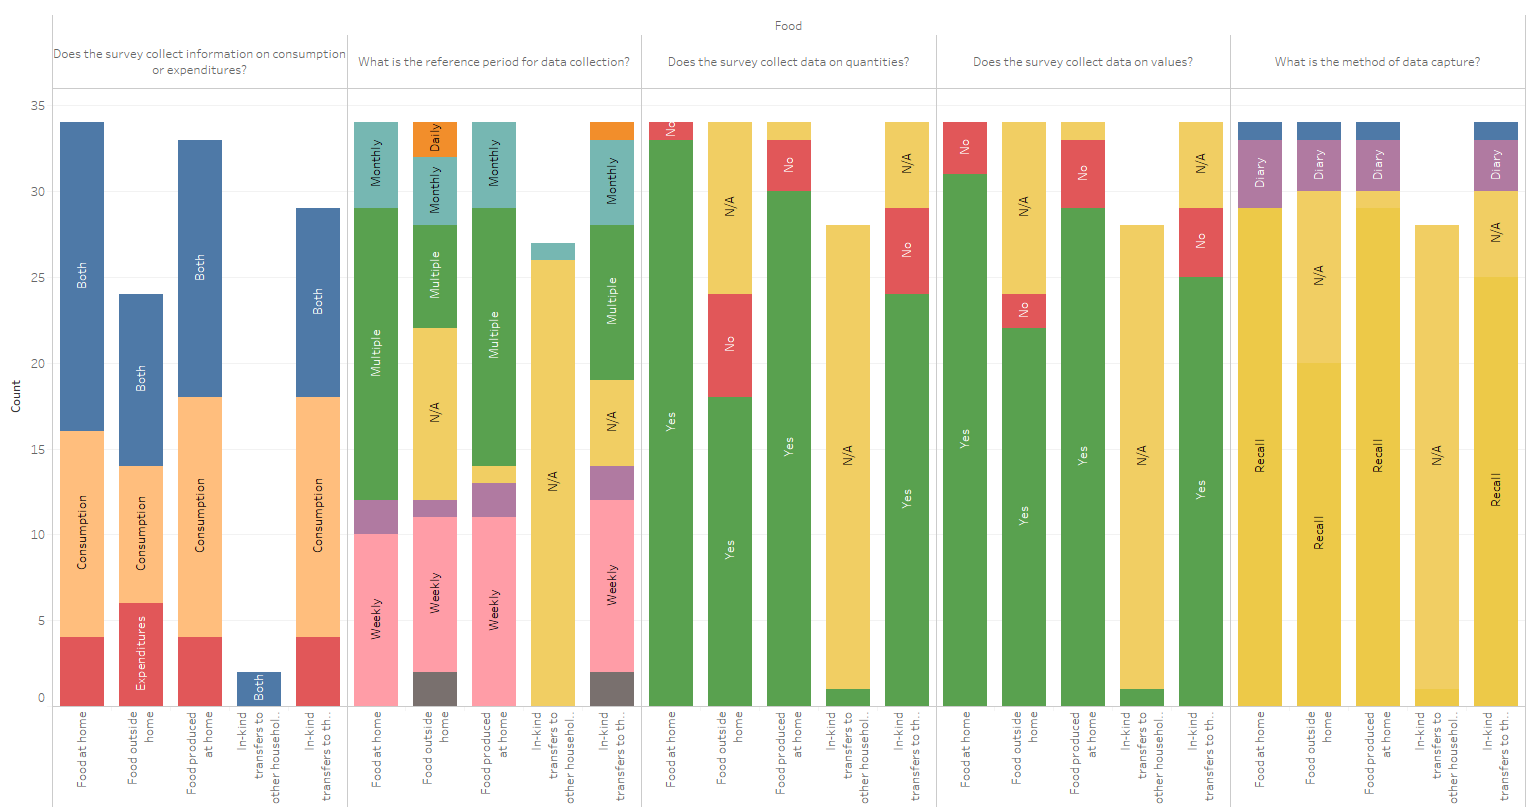
\includegraphics{figures/Food.png}}

\subsection{Non-food}\label{non-food}

The second component, non-food expenditures, includes frequently
purchased goods and services like soap, cleaning supplies, newspapers,
and personal care items. It also includes some less frequent but regular
purchases items like clothing, footwear, kitchen equipment, curtains,
bedcovers, etc. In most cases, the non-food expenditures component must
be constructed by aggregating expenditures on goods and services from
different sections of a survey.

A homogenous definition of what constitutes non-food expenditures is
required. The Classification of Individual Consumption According to
Purpose (COICOP) is the international reference classification for
household expenditures. We define non-food expenditures as categories
2-12 of the COICOP:

\begin{enumerate}
\def\labelenumi{\arabic{enumi}.}
\tightlist
\item
  Food and non-alcoholic beverages
\item
  Alcoholic beverages, tobacco and narcotics
\item
  Clothing and footwear
\item
  Housing, water, electricity, gas and other fuels
\item
  Furnishings, household equipment and routine household maintenance
\item
  Health
\item
  Transport
\item
  Information and communication
\item
  Recreation, sport and culture
\item
  Education services
\item
  Restaurants and hotels
\item
  Miscellaneous goods and services
\end{enumerate}

In Bangladesh 2016, non-food expenditures included fuel and lightning,
cosmetics and hygiene items, transport and travel, ready-made garments,
clothing materials, footwear, household-use textiles, health treatment
expenses, housing related expenses, education, recreation and leisure.
In Bhutan 2017, non-food expenditures included tobacco and doma,
clothing and footwear, transport and communications, household
operations, recreation, furnishings and household equipment,
agricultural input and machinery, miscellaneous expenditure, educational
expenses, health expenses, rental expenses, energy for the home, and
remittances abroad.

Similarly to what found studying the food component, non-food items are
also collected for different reference periods, for example, from
consumption in the last 30 days, past 3 months, or the last year.
Monthly is the most frequent collection period for non-food
expenditures. Both food and non-food expenditures have insufficient
coverage on transfers.

\begin{table}[t]

\caption{\label{tab:nonfood}Non-Food}
\centering
\begin{tabular}{lllll}
\toprule
Country, Year & Number of non-food items & Collection method & Quantity and/or Value & Transfers\\
\midrule
Afghanistan, 2016 & NA & NA & NA & NA\\
Bangladesh, 2016 & NA & NA & NA & NA\\
Bhutan, 2017 & NA & NA & NA & NA\\
India, 2017 & NA & NA & NA & NA\\
Maldives, 2016 & NA & NA & NA & NA\\
\addlinespace
Nepal, 2016 & NA & NA & NA & NA\\
Pakistan, 2015 & NA & NA & NA & NA\\
Sri Lanka, 2016 & NA & NA & NA & NA\\
\bottomrule
\end{tabular}
\end{table}

We provide a
\href{https://tab.worldbank.org/\#/site/WBG/views/SAR_MNA_Metadata/NonFood}{Tableau
Dashboard} where the user may compare surveys according to:

\begin{itemize}
\tightlist
\item
  The number of
  \href{https://tab.worldbank.org/\#/site/WBG/views/SAR_MNA_Metadata/Items}{non-food
  items} in the non-food basket
\item
  Whether they collect the quantity and/or value of non-food items
\item
  Data collection reference periods (daily, weekly, bi-weekly, monthly,
  and/or yearly)
\item
  Whether they provide information on transfers to and from the
  household
\end{itemize}

\href{https://tab.worldbank.org/\#/site/WBG/views/SAR_MNA_Metadata/NonFood}{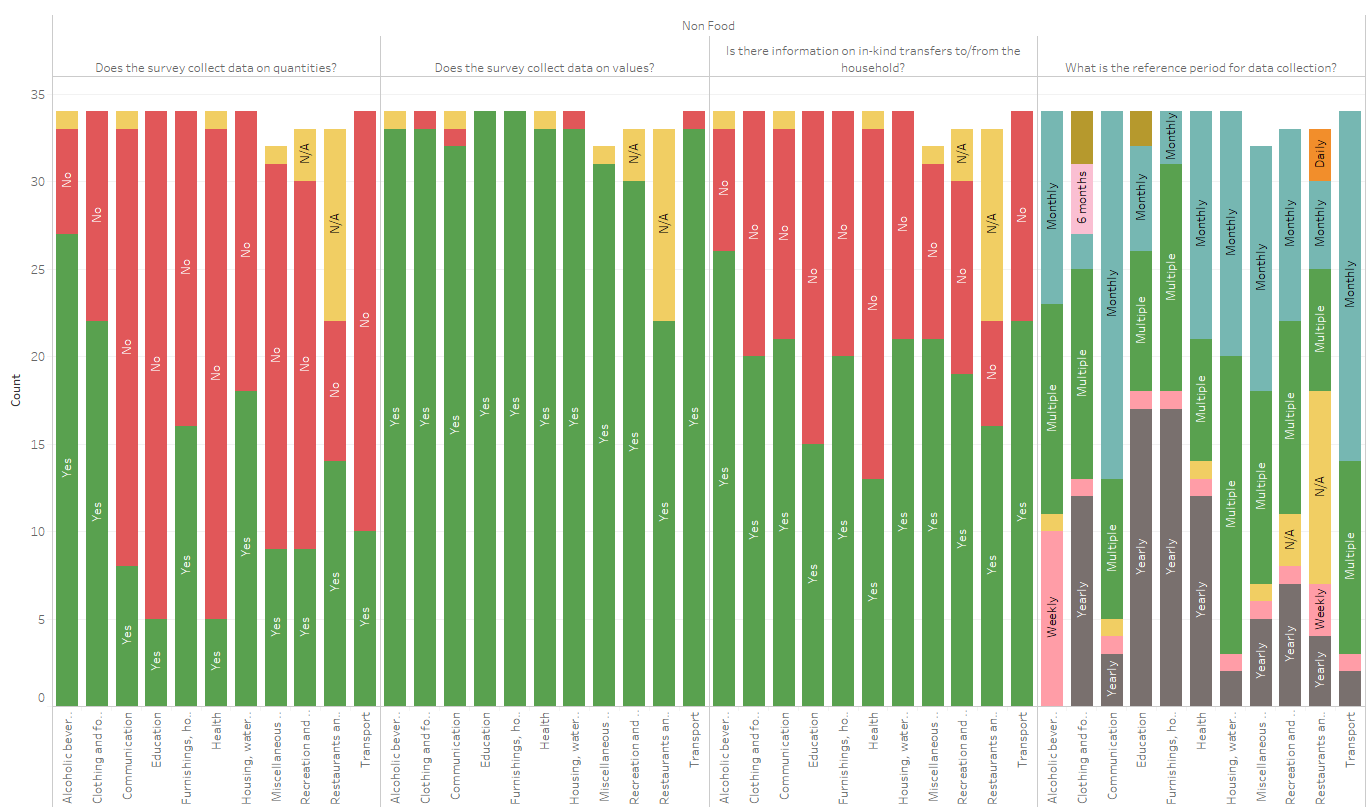
\includegraphics{figures/Nonfood.png}}

\subsection{Durable assets}\label{durable-assets}

The third component is consumer flows from durable assets. The consumer
flows (also referred to as user costs or rental equivalents) of durable
assets represent the opportunity cost of money invested in these goods
taking into account their lifetime and depreciation. The most important
finding regarding the collection of data on durable assets through
household surveys in South Asia is that the data collection methods
followed can be very different. This section provides a summary for data
collection methods for durable assets for the household surveys
available in SARMD.

It is expected for data collection methods to vary over time and from
one country to another. However, even for items within a country's
particular survey we can see different data collection methods. For
example, even though both cows and cars may be considered productive
assets, the information available for these two assets within a survey
may be very different and would be contained in different sections of
the survey. Even for more similar goods, like a washing machine and a
sewing machine, the information provided by a survey may differ. For
that reason, we found it necessary to characterize each item's data
collection method separately. Data available for household assets
(e.g.~a car) may be different from data available for agricultural
assets (e.g.~a tractor). Some assets are grouped together, while others
are collected individually, and some may even have their own section in
the survey. This is the case for cellphones, which are durable assets,
but are usually given special treatment and collected separately in the
surveys.

Long-lived goods (automobiles, appliances, furniture) have a positive
and significant impact on living standards. These durable assets may
deliver useful services to consumers through repeated use over an
extended period of time. For that reason, surveys should collect data on
all assets available to the household, not just the ones purchased
recently. This is unfortunately the case for India 2011 and Pakistan
2015. Pakistan 2015 asks only if items were purchased in the last year.
India 2011 only collects specific details for those assets acquired in
the last 30 days or in the last year.

To measure the flows from using durable goods over extended periods of
time, we need to know their quantity, date of purchase, and how much
they cost at the time of purchase vs.~their current value. Nepal AHS
2016 represents the standard practice a survey should follow. Nepal AHS
2016 asks whether the assets are available, their quantity, age,
purchase and current values, and whether the assets were paid for or
received as gift. Asking how many years ago was an asset acquired
provides more information than asking whether the asset was purchased in
the last 12 months. The most incomplete example would have to be
Pakistan 2015, which focuses only on assets acquired in the last year
and only measures values, not quantities.

Table \ref{tab:durables} provides a quick comparison between countries
by presenting the number of assets collected, and their collection
method (i.e.~quantity and/or value). In addition, we provide a
\href{https://tab.worldbank.org/\#/site/WBG/views/SAR_MNA_Metadata/Durables}{Tableau
dashboard} where the user may identify which surveys collect
insufficient information regarding durable assets.

\begin{table}[t]

\caption{\label{tab:durables}Durables}
\centering
\begin{tabular}{lrll}
\toprule
Country, Year & Number of assets & Quantity & Value\\
\midrule
Afghanistan, 2016 & 18 & Yes & Yes\\
. & 7 & Yes & Yes\\
Bangladesh, 2016 & 27 & Yes & Yes\\
Bhutan, 2017 & 13 & No & No\\
. & 9 & Yes & No\\
\addlinespace
. & 23 & Yes & Yes\\
India, 2011 & 53 & Yes, but only if recently purchased & Yes, but only if recently purchased\\
Maldives, 2016 & 16 & Yes & Yes\\
Nepal, 2016 & 23 & Yes & Yes\\
Pakistan, 2015 & 67 & No & Yes, but only if recently purchased\\
\addlinespace
Sri Lanka, 2016 & 25 & Yes & Yes\\
\bottomrule
\end{tabular}
\end{table}

\href{https://tab.worldbank.org/\#/site/WBG/views/SAR_MNA_Metadata/Durables}{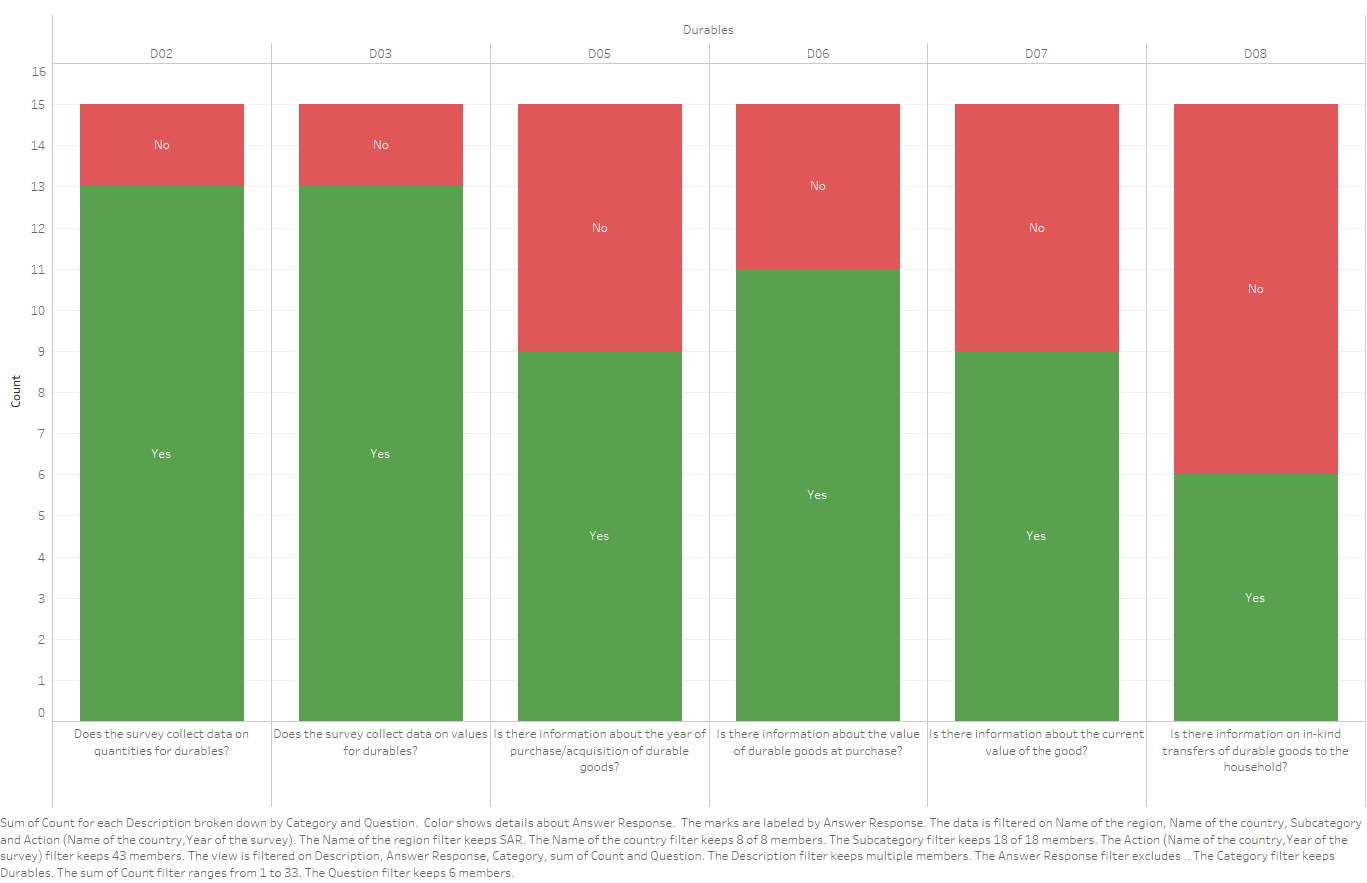
\includegraphics{figures/Durables.png}}

\subsection{Housing}\label{housing}

The fourth component is rent, which is in some cases observed directly
for households who rent their house or apartment. For the rest, rent is
obtained either by asking a household how much you would expect to
receive each month for this house if you rented it out to someone, or by
using a hedonic housing regression model based on dwelling
characteristics and actual rent or house values. Therefore, there are
three types of rent:

\begin{enumerate}
\def\labelenumi{\arabic{enumi}.}
\tightlist
\item
  Rent paid by households when they are not owners of their dwelling:
  i.e.~How much do you pay per month?
\item
  Self-reported or imputed rent by households who are owners of their
  dwelling: i.e.~How much do you think you would have to pay if you had
  to rent this dwelling?
\item
  Predicted rent by households who are owners of their dwelling and did
  not self-report their rent: i.e.~How much does the hedonic regression
  model predict a household would have to pay for a dwelling of these
  characteristics?
\end{enumerate}

Most households in South Asia do not report values on paid rent because
most households are owners of housing rather than renters. One area of
South Asia where we find low levels of house ownership is Thimphu in
Bhutan. According to Bhutan LSS 2017, in Thimphu, 59\% of the households
pay rent, while 17\% of households live in rent-free dwellings. Of
rent-paying households, 85\% live in dwellings owned by private
individuals and 14\% live in housing owned by the government and by
public corporations.

The methodologies for a hedonic regression model vary by country. The
methodology followed by Afghanistan differs from the rest of the
countries in that they base their hedonic pricing model on the
dwelling's values and then convert it to a monthly rent, instead of
trying to directly estimate rents. In Afghanistan, actual rent for
renters is collected by asking ``How much money per month does your
household pay to live in this dwelling?''. However, there is a low
number of renters. Self-reported rent was not included in the survey.
Instead, rents are predicted by a hedonic regression model. Half of all
owners in the LCS 2016 report the value of their dwelling by answering
``If you were to purchase this dwelling today, how much would it
cost?''. For these households, a hedonic housing model is estimated and
used to predict the value of the dwelling based on the characteristics
of the dwelling. A hedonic housing model relates the housing price to
factors such as size, location, construction materials, etc. Separate
regressions are estimated for urban, rural and tent dwellings. The
actual or predicted housing values are converted to a monthly rent by
imposing a relationship based on interest and depreciation rates. For
ALCS 2016 a depreciation rate of 1.5 percent and an interest rate of 2.5
percent are assumed.

For Bangladesh HIES 2016, the housing expenditure component may include
the three types or rent depending on the homeownership status of each of
the households: actual rent, imputed rent (i.e., the amount that
homeowners report they would like to get if they could rent their house)
or predicted rent. For households that did not report rent or
self-report their rent, a predicted rent was estimated using a hedonic
regression model. This regression model was estimated using the (log of)
reported rent on the left-hand side and was regressed against a set of
housing characteristics, including number of rooms, wall materials,
access to electricity and tap water, kitchen, dining room, telephone
connection, dwelling's land size, and a vector of the 16 original strata
dummy variables. The value of dwellings was collected by asking ``If you
want to buy or construct a dwelling just like this today, how much money
would you have to pay?'', but it is not clear whether this value was
used in the hedonic regression model.

In the rest of the countries, households are asked for their
hypothetical rental values, not for the value of their dwelling. Table
\ref{tab:housing} summarizes how each survey collects rent or dwelling
values for households who own their dwelling. For Bhutan LSS 2017,
households were asked about the amount of rent they pay for their
dwelling in a month. People who own their dwelling or stay in rent-free
houses were asked to estimate the monthly house rent for their
dwellings. The question was ``How much would you pay if you had to rent
this dwelling?''. A similar question is included in the surveys Maldives
HIES 2016, Nepal AHS 2016 and Sri Lanka HIES 2016. India 2011 and
Pakistan 2015 still lack enough data to measure rents.

\begin{table}[t]

\caption{\label{tab:housing}Housing}
\centering
\begin{tabular}{ll}
\toprule
Country, Year & How is rent calculated for owners?\\
\midrule
Afghanistan, 2016 & If you were to purchase this dwelling, how much would it cost?\\
Bangladesh, 2016 & Imputed rent; also asks If you want to buy or construct a dwelling just like this today, how much money would you have to pay?\\
Bhutan, 2017 & How much do you think you would have to pay if you had to rent this dwelling?\\
India, 2011 & NA\\
Maldives, 2016 & How much would you expect to receive each month for this house if you rented it out to someone?\\
\addlinespace
Nepal, 2016 & If any person want to take this house in rent, how much money would have to pay?\\
Pakistan, 2015 & NA\\
Sri Lanka, 2016 & What is the estimated rent of owner-occupied house?\\
\bottomrule
\end{tabular}
\end{table}

The most relevant dwelling characteristics displayed in the
\href{https://tab.worldbank.org/\#/site/WBG/views/SAR_MNA_Metadata/Housing}{Tableau
dashboard} are:

\begin{itemize}
\tightlist
\item
  Rent captured by households' reported rent or estimated by fitting a
  hedonic pricing model (regressing information available on housing
  characteristics on housing values)
\item
  Type of dwelling (house, part of house, separate apartment, shared
  apartment)
\item
  Tenure status
\item
  Area of dwelling, number of bedrooms, bathrooms, and kitchen
\item
  Material of the walls, roof, and floor
\item
  Sources of drinking water
\item
  Sanitation (access to flush toilet, pit latrine)
\item
  Access to electricity
\item
  Travel time to reach services
\item
  Others such as access to an Internet connection
\end{itemize}

\href{https://tab.worldbank.org/\#/site/WBG/views/SAR_MNA_Metadata/Housing}{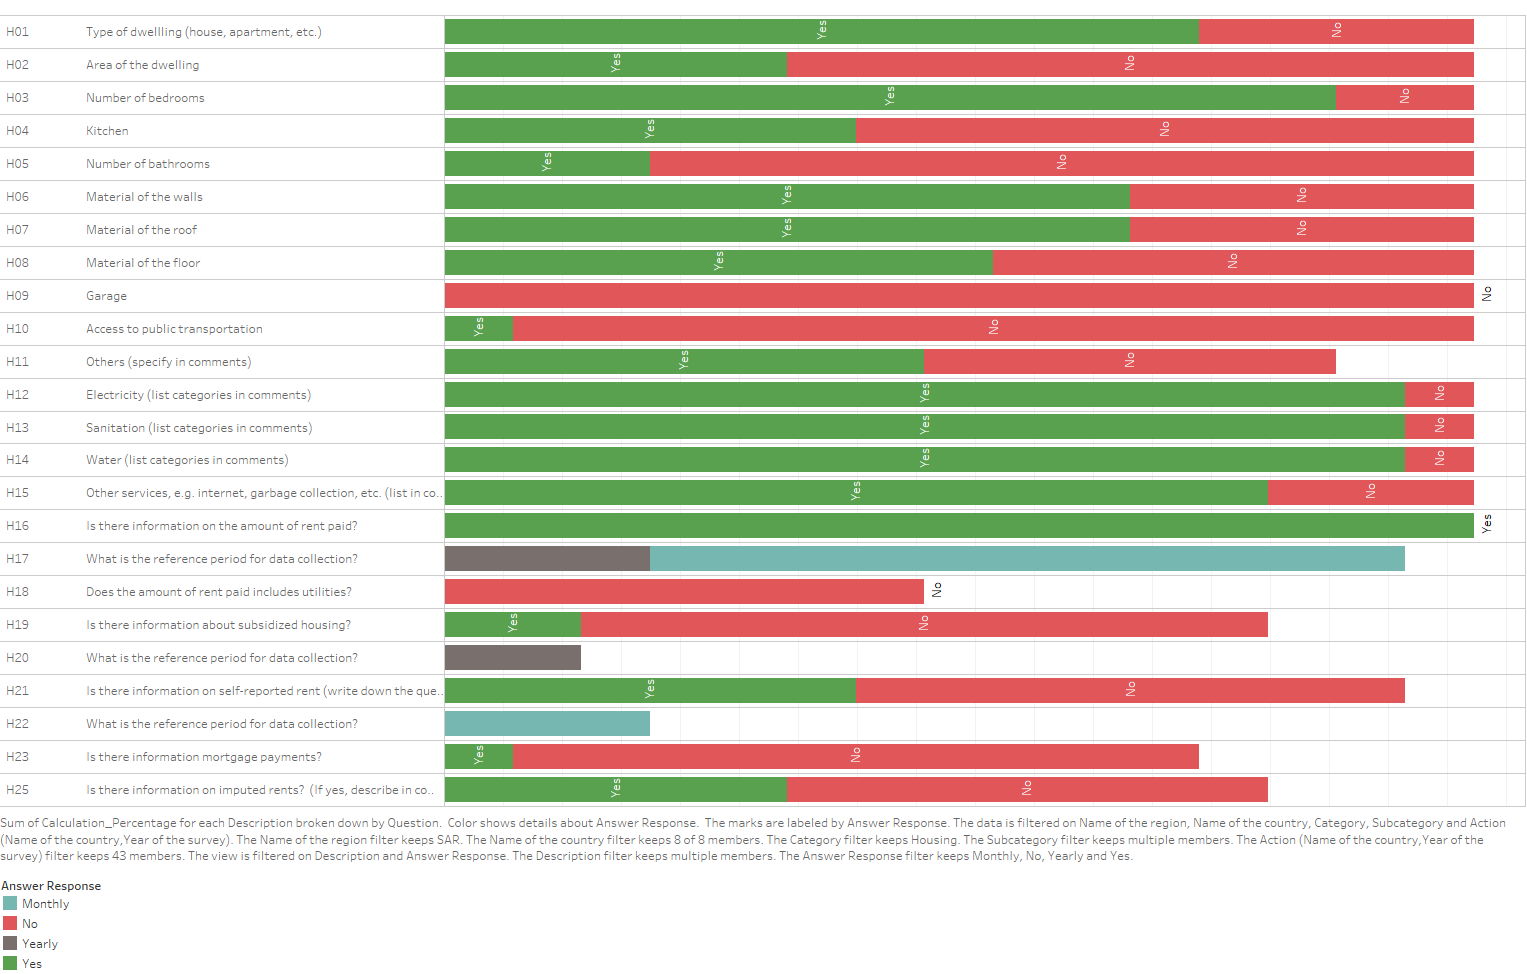
\includegraphics{figures/Housing.png}}

\part{Quality Check}\label{part-quality-check}

\chapter{Harmonized variables}\label{qcheck}

\begin{Shaded}
\begin{Highlighting}[]
\NormalTok{**STATA Example**}

\FunctionTok{# Opening a dataset in SARMD}
\NormalTok{datalibweb, country(BGD) years(2016) type(SARMD) clear}
\end{Highlighting}
\end{Shaded}

\begin{center}\rule{0.5\linewidth}{\linethickness}\end{center}

This chapter presents the harmonized data from the South Asia Micro
Database (SARMD) with a series of quality checks to verify that each
harmonized variable has been constructed properly. Two kinds of quality
checks of the harmonized data have been conducted. A static quality
check evaluates whether the harmonized variables are present and whether
there is a high percentage of missing values. It also delves deeper into
variables that may be interrelated with other variables. For example, a
high percentage of households that have access to a television, but do
not have access to electricity may raise questions on how these
variables were constructed. A dynamic quality check evaluates the
inconsistencies in measurement of harmonized data over time. It provides
a better overview on whether categorical variables have changed over
time and provides poverty and inequality measures.

\section{Basic survey
characteristics}\label{basic-survey-characteristics}

\begin{longtable}[]{@{}rrrr@{}}
\toprule
countrycode & veralt & pop\_wgt & subnatid2\tabularnewline
\midrule
\endhead
year & idh & int\_year & psu\tabularnewline
survey & idp & int\_month & strata\tabularnewline
vermast & wgt & subnatid1 & spdef\tabularnewline
\bottomrule
\end{longtable}

The essential variables that identify each dataset and should always be
included are \textbf{countrycode}, \textbf{year}, \textbf{survey},
\textbf{vermast}, \textbf{veralt}, \textbf{idh}, and \textbf{idp}.
Weights are defined as \textbf{wgt} and \textbf{pop\_wgt=wgtxhsize}. The
dates of the survey are recorded as \textbf{int\_year} and
\textbf{int\_month}. The geographical location within the country's
administrative division is recorded as \textbf{subnatid1}, and in some
cases, \textbf{subnatid2} may provide a more specific location.
\textbf{psu} \textbf{strata} \textbf{spdef}

\section{Demographics}\label{demographics}

\begin{longtable}[]{@{}rrr@{}}
\toprule
age & male & hsize\tabularnewline
\midrule
\endhead
relationcs & relationharm & marital\tabularnewline
\bottomrule
\end{longtable}

Demographic variables consist of \textbf{age}, \textbf{male},
\textbf{hsize}, \textbf{relationcs}, \textbf{relationharm} and
\textbf{marital}. Household size is close to seven in Afghanistan,
Pakistan and Maldives, and much closer to 4-5 in the rest of the
countries. Population pyramids such as the one provided in Figure
\ref{fig:pyramid} allow to see how countries' demographics change over
time while showing whether the marital status of individuals has been
harmonized adequately.

\begin{Shaded}
\begin{Highlighting}[]
\NormalTok{knitr::}\KeywordTok{include_graphics}\NormalTok{(}\StringTok{"figures/Pyramid.png"}\NormalTok{)}
\end{Highlighting}
\end{Shaded}

\begin{figure}

{\centering 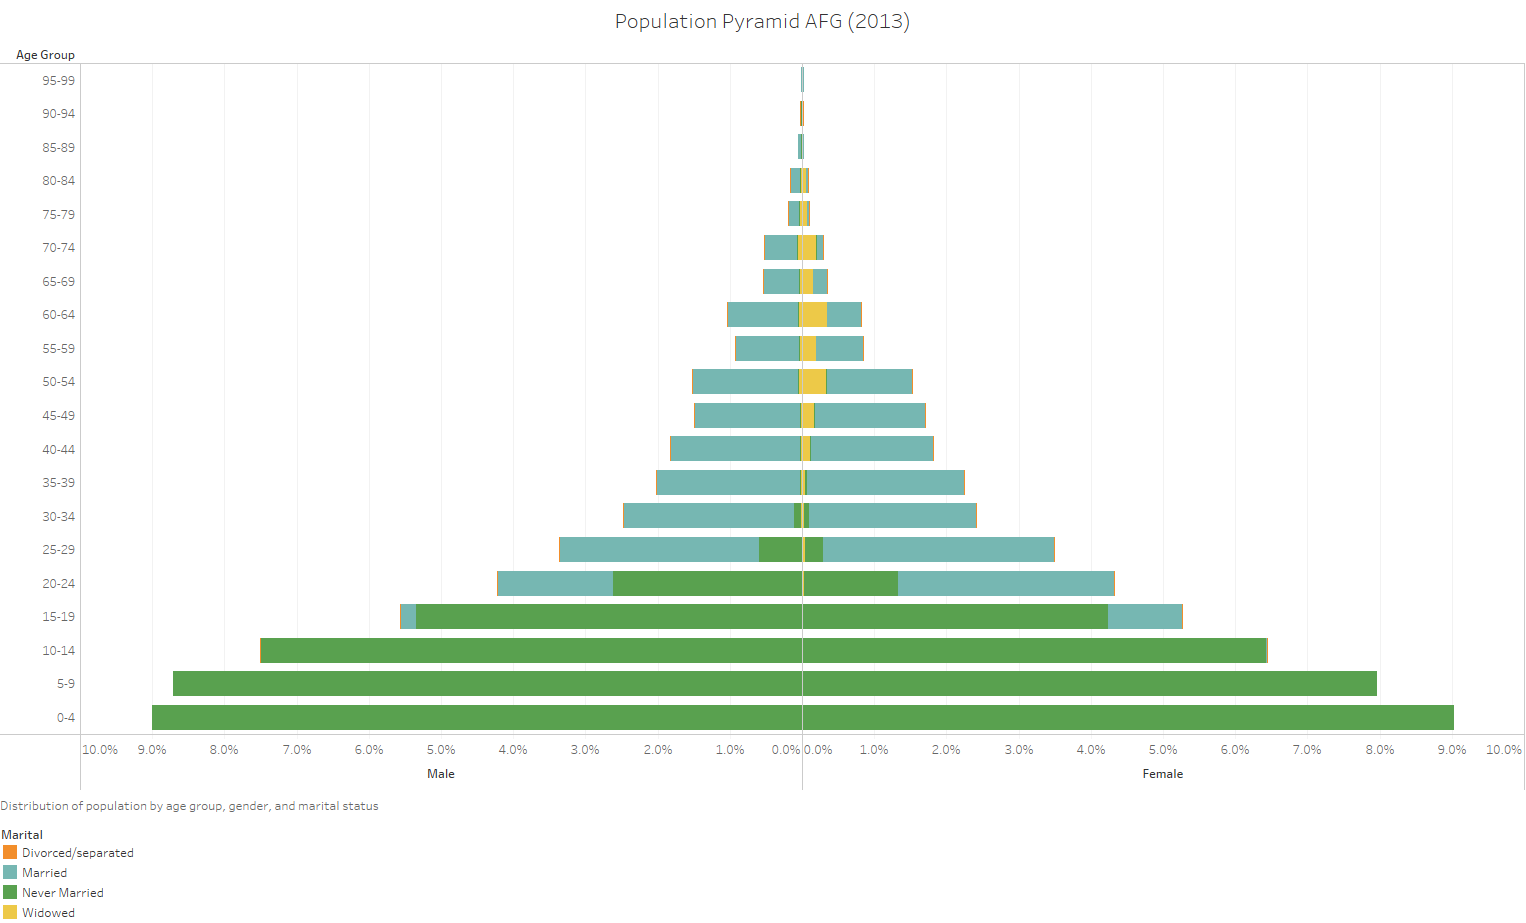
\includegraphics[width=0.8\linewidth]{figures/Pyramid} 

}

\caption{Population Pyramid for Afghanistan (2013)}\label{fig:pyramid}
\end{figure}

see Figure \ref{fig:pyramid} at
\url{https://tab.worldbank.org/\#/site/WBG/views/SAR_MNA_Demographics/Pyramid}

\section{Education}\label{education}

\begin{longtable}[]{@{}rrrr@{}}
\toprule
atschool & ed\_mod\_age & everattend & literacy\tabularnewline
\midrule
\endhead
educat4 & educat5 & educat7 & educy\tabularnewline
\bottomrule
\end{longtable}

The adult literacy rate -- referring to the population aged 15 and over
-- is an indicator that measures the accumulated achievement of the
education system. The youth literacy rate -- the literacy rate in the
population aged 15-24 -- reflects the outcomes of primary education over
roughly the previous 10 years and is a measure of recent educational
progress.

\section{Durable assets}\label{durable-assets-1}

\begin{longtable}[]{@{}rrrr@{}}
\toprule
bicycle & computer & landphone & refrigerator\tabularnewline
\midrule
\endhead
buffalo & cow & motorcar & sewing machine\tabularnewline
cellphone & fan & motorcycle & television\tabularnewline
chicken & lamp & radio & washing machine\tabularnewline
\bottomrule
\end{longtable}

This section analyzes whether the sixteen asset variables in SARMD have
been adequately harmonized and may be used for research purposes. These
binary variables (Yes=1, No=0) represent whether households have access
to a particular durable asset. The variables are defined at the
household level and do not represent whether each individual owns an
asset in particular, but whether the household as a whole has access to
it. The harmonization of these asset variables is limited by their
availability in the household questionnaire. For example, cow, chicken,
and buffalo cannot be harmonized if a survey does not cover
live-stocking activities. It may also be that some of these assets are
unnecessary (a fan in cold weather), obsolete (land phone), or too basic
(lamp) to be included in a questionnaire.

Quality checks were conducted to make sure that these variables could
only be equal to 0 or 1. We also verified that the value was the same
within each household. A deeper look at these asset variables allowed to
identify some interesting trends. Figure \ref{fig:assets} displays the
percentage of households that have access to an asset by country for the
latest survey round available. It shows that cellphones are the most
accessible assets and that there can be a wide range between the minimum
and the maximum.

\begin{Shaded}
\begin{Highlighting}[]
\NormalTok{knitr::}\KeywordTok{include_graphics}\NormalTok{(}\StringTok{"figures/Assets.png"}\NormalTok{)}
\end{Highlighting}
\end{Shaded}

\begin{figure}

{\centering 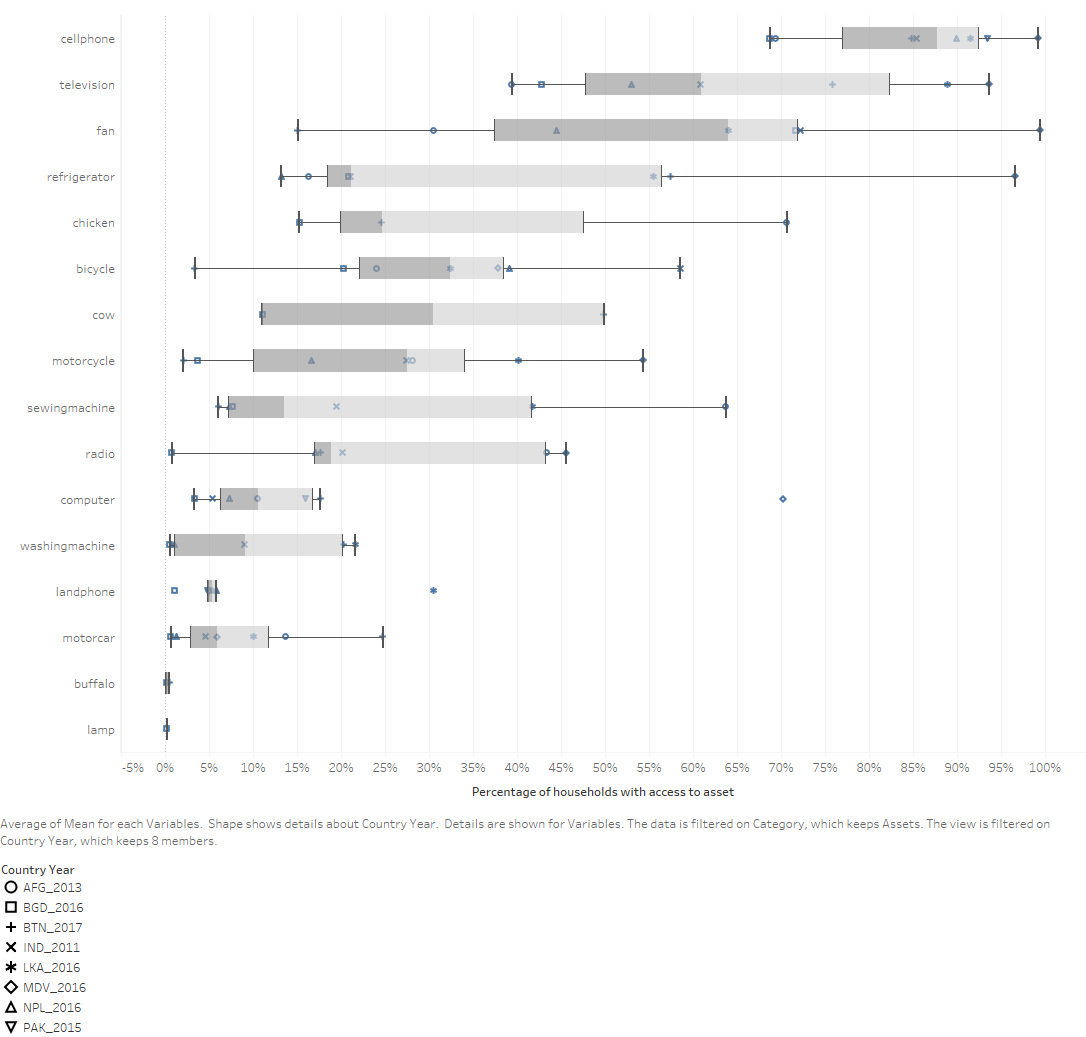
\includegraphics[width=0.8\linewidth]{figures/Assets} 

}

\caption{Harmonized asset ownership in latest household survey round}\label{fig:assets}
\end{figure}

see Figure \ref{fig:assets} at
\url{https://tab.worldbank.org/\#/site/WBG/views/SAR_MNA_Summary/Assets}

\begin{Shaded}
\begin{Highlighting}[]
\NormalTok{knitr::}\KeywordTok{include_graphics}\NormalTok{(}\StringTok{"figures/Scatter.png"}\NormalTok{)}
\end{Highlighting}
\end{Shaded}

\begin{figure}

{\centering 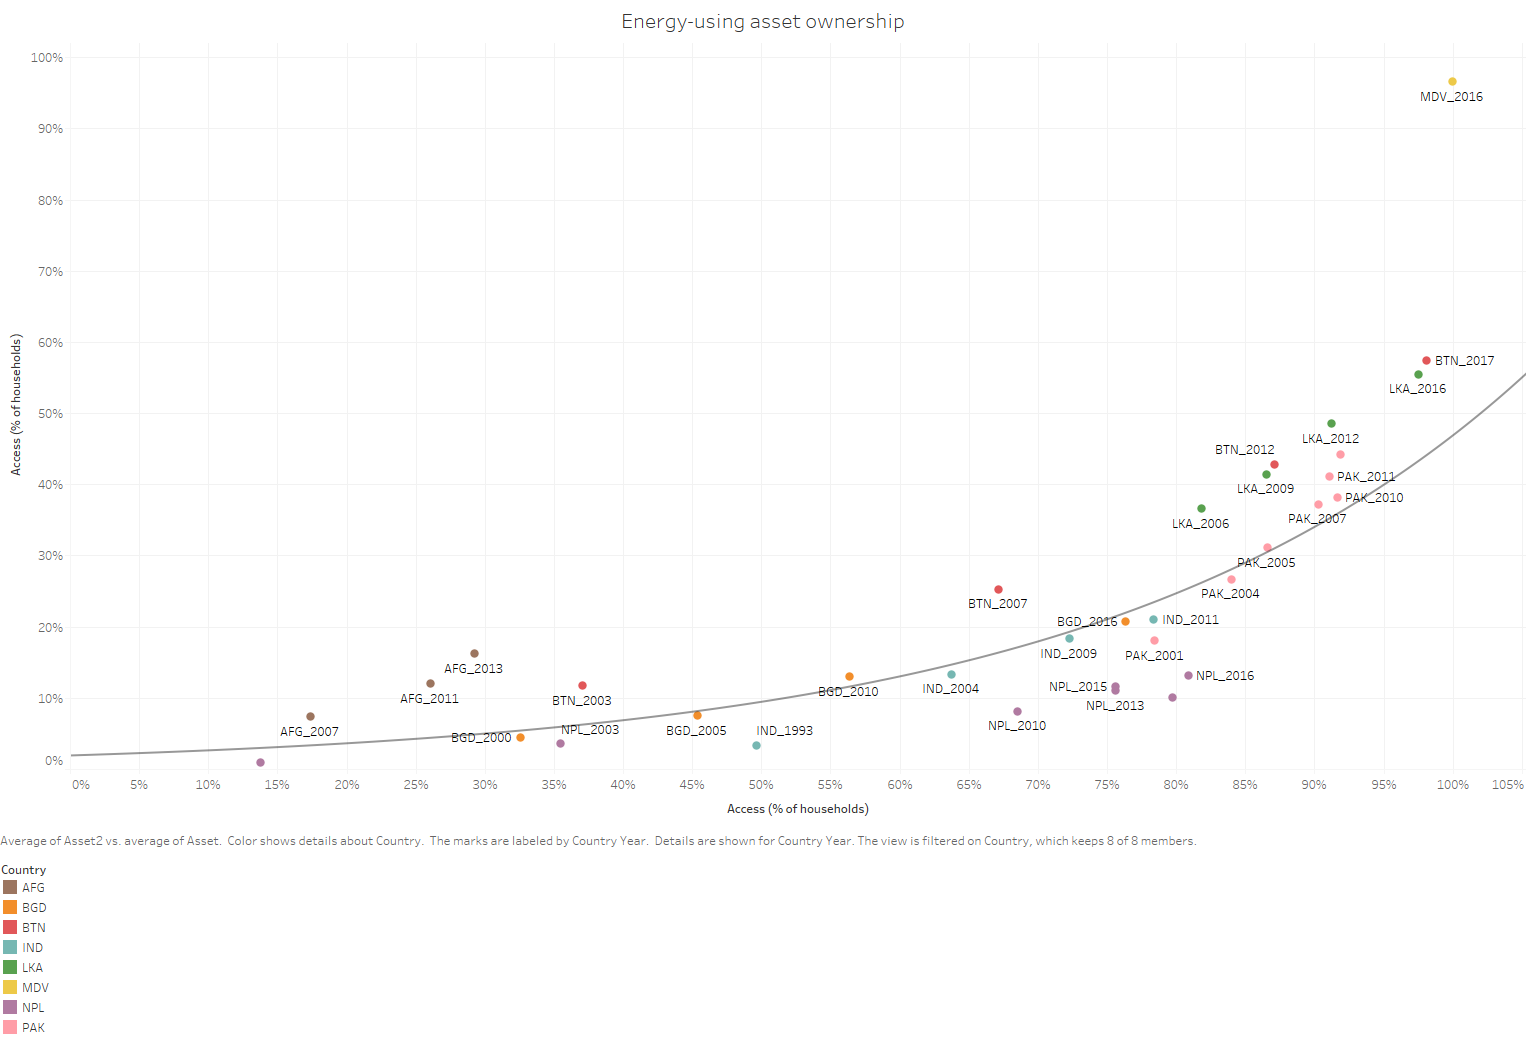
\includegraphics[width=0.8\linewidth]{figures/Scatter} 

}

\caption{Access to refrigerator and access to electricity across surveys}\label{fig:scatter}
\end{figure}

see Figure \ref{fig:scatter} at
\url{https://tab.worldbank.org/\#/site/WBG/views/SAR_MNA_Summary/Scatter}

Figure \ref{fig:scatter} shows a clear exponential trend between the
percentage of households that have access to electricity and the
percentage of households that have access to a refrigerator. A similar
relationship with electricity was found for television, washing machine,
and fan. A quality check was conducted to identify the number of
observations where the household had no access to electricity, but still
had access to an asset. In some cases, it might seem illogical, for
example, for a household to own a television if it does not have access
to electricity. In Afghanistan (2013), 7,771 out of 20,773 households
seemed to have a television and no electricity. However, a mistake in
the harmonization process was identified and this number was reduced to
3,119 out of 20,773 households once the mistake was fixed. Still,
13-20\% of observations in Afghanistan have consistently reported having
a television and no electricity.

\section{Housing}\label{housing-1}

The living conditions of the Afghan population are to a large extent
determined by the conditions of housing, including facilities for
drinking water and sanitation. Most people -- 83 percent -- live in
dwellings that are constructed with non-durable materials and 44 percent
live in conditions of overcrowding, meaning that there are more than
three persons per room. The large majority of urban dwellers -- 72
percent -- live in slums or inadequate housing.

\section{Labor}\label{labor}

\section{Poverty}\label{poverty}

This section presents the latest data on regional extreme poverty rates
using the international poverty line of US\$1.90 in 2011 purchasing
power parity dollars. Even though, Afghanistan is missing, the ALCS
2016-17 recorded a sharp deterioration in welfare of the Afghan
population. The proportion of population living below the national
poverty line increased from 34 percent in 2007-08 to 55 percent in
2016-17. The latest poverty figures imply that at the time of the
survey, close to 16 million Afghans lived in poverty.

Urban poverty lower than rural poverty.

datalibweb, country(PAK) year(2015) type(GMD) mod(ALL) vermast(01)
veralt(02) surveyid(PSLM) gen welf\_ppp = welfare/cpi2011/icp2011/365
gen poor190 = welf\_ppp \textless{} 1.9 sum poor190 {[}aw=weight\_h{]}

\section{Inequality}\label{inequality}

The Gini index for Afghanistan showed a small decrease between the
surveys of 2011-12 and 2016-17, from 0.30 to 0.29.

\part{Analytical notes}\label{part-analytical-notes}

\chapter{Analytical notes}\label{application}

\begin{center}\rule{0.5\linewidth}{\linethickness}\end{center}

Some \emph{significant} applications are demonstrated in this chapter.

\section{School attendance by age}\label{school-attendance-by-age}

\section{Household composition and
expenditures}\label{household-composition-and-expenditures}

Figure \ref{fig:children} shows how average household size declines as
we move to higher quintiles of per capita expenditures. Average
household size is 9.66 in the poorest per capita expenditure quintile of
Afghanistan, compared to 3.91 in the richest per capita expenditure
quintile of Sri Lanka. Having more children (individuals \textless{} 15
years old) is negatively correlated with household per capita
expenditures. We would expect higher poverty rates among large
households and households with more children.

\begin{Shaded}
\begin{Highlighting}[]
\NormalTok{knitr::}\KeywordTok{include_graphics}\NormalTok{(}\StringTok{"figures/Children.png"}\NormalTok{)}
\end{Highlighting}
\end{Shaded}

\begin{figure}

{\centering 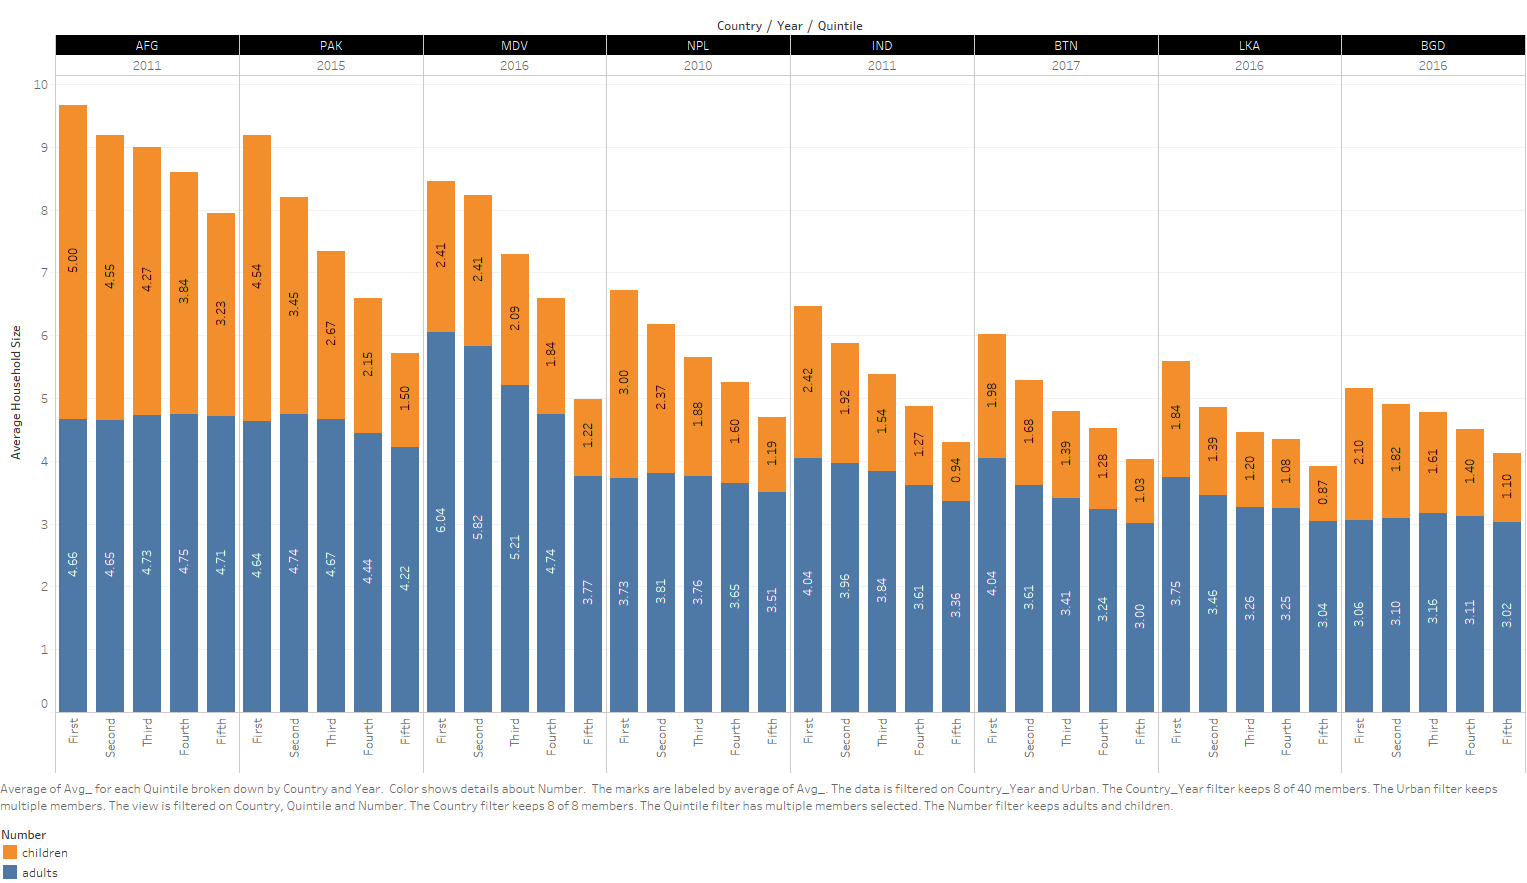
\includegraphics[width=0.8\linewidth]{figures/Children} 

}

\caption{Average household size by per capita consumption quintile}\label{fig:children}
\end{figure}

see Figure \ref{fig:children} at
\url{https://tab.worldbank.org/\#/site/WBG/views/SAR_MNA_Demographics/Children}

\section{Gender inequality in
literacy}\label{gender-inequality-in-literacy}

The most vulnerable group in terms of low literacy is women older than
65 years. Even among younger adults and children, the difference in
literacy rates between men and women is wide. Afghanistan has one of the
lowest literacy rates in the world. In 2011, it was estimated at about
31\% of the adult population (15 years or older).

\begin{Shaded}
\begin{Highlighting}[]
\NormalTok{knitr::}\KeywordTok{include_graphics}\NormalTok{(}\StringTok{"figures/Literacy.png"}\NormalTok{)}
\end{Highlighting}
\end{Shaded}

\begin{figure}

{\centering 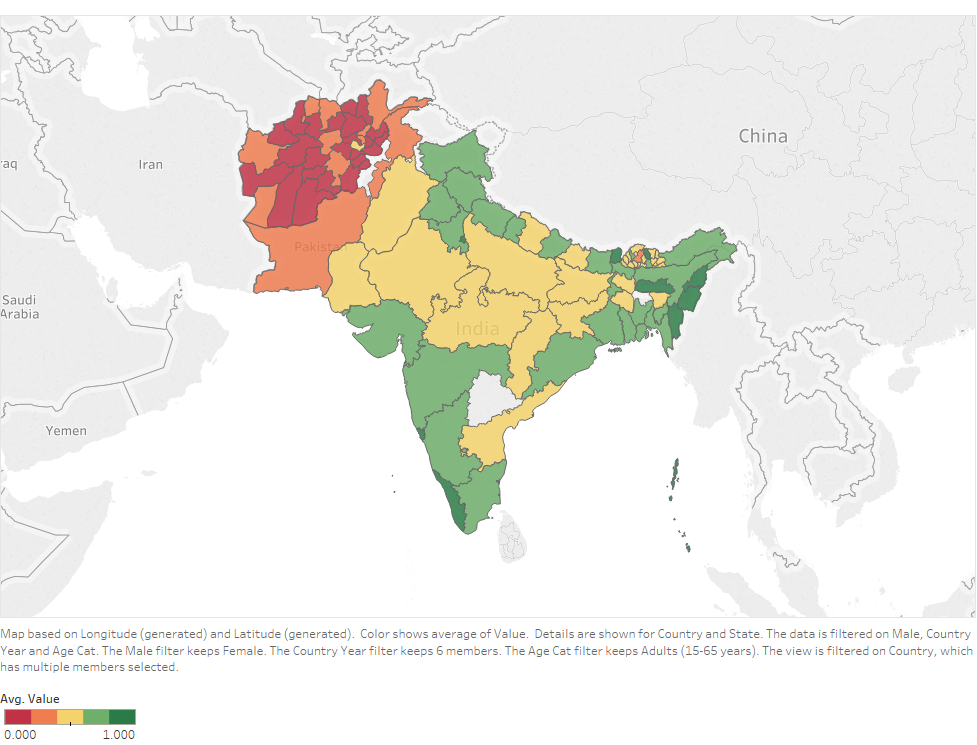
\includegraphics[width=0.8\linewidth]{figures/Literacy} 

}

\caption{Female Literacy Rate (15-65 years)}\label{fig:literacy}
\end{figure}

see Figure \ref{fig:literacy} at
\url{https://tab.worldbank.org/\#/site/WBG/views/Note3/Literacy}

\section{Nonlinear relationship between expenditure and asset
acquisition}\label{nonlinear-relationship-between-expenditure-and-asset-acquisition}

Energy-using appliances, such as refrigerators, are taken for granted
among households in developed countries. However, in developing
countries these assets are still scarce and owning a refrigerator can
have important consequences on the well-being of a family. This note
explains who owns this kind of assets in South Asia with the use of
harmonized data from SARMD. Refrigerators, for example, can be common in
urban areas of New Delhi and be virtually non-existent in central
Afghanistan. The distribution of assets among the population is an
indicator in the fight against extreme poverty. Even in developed
countries, the possession of valuable assets that facilitate family
labor in a meaningful way are quick indicators of economic development
in a region and the purchasing power of households.

\url{https://tab.worldbank.org/\#/site/WBG/views/Note1/Dashboard1}

An estimated 368 million people live without electricity in their homes
in South Asia, and even among those who have access, many do not own
basic assets such as refrigerators, televisions, or washing machines. We
study household decisions to acquire assets in the presence of rising
incomes. Table ?? demonstrates the low penetration that these
energy-consuming assets have in South Asia. As more households currently
living in poverty benefit from overall economic development, we would
expect a considerable increase in households' energy use. If one half of
the households in India who do not own refrigerators were to buy one,
annual nationwide electricity demand would rise by over 10 percent
(Wolfram, Shelef, and Gertler 2012).

We model the nonlinear relationship between income and asset acquisition
as in Gertler, Shelef, Wolfram \& Fuchs (2016). This paper provides a
simple theoretical framework to characterize the effect of income growth
on asset purchases when consumers face credit constraints. A nonlinear
Engel curve means that as income goes up from initially very low levels,
credit-constrained households do not immediately become more likely to
purchase an energy-using asset. Households faced with credit constraints
become much more likely to purchase energy-using assets with once their
income passes a threshold level. We begin by documenting an S-shaped
relationship between expenditure and durable asset ownership. Figure 1
plots the share of households that own refrigerators, televisions, and
washing machines in India (2011) against household expenditure.

Figure ?? demostrates how for a group of several assets, asset ownership
is high in the Maldives and lower in the rest of South Asia. Filmer and
Pritchett, 2001, argue that the first principal component of the
household's ownership of physical assets is highly correlated with
household expenditure and can be used as a reasonable proxy.

\chapter*{References}\label{references}
\addcontentsline{toc}{chapter}{References}

\begin{center}\rule{0.5\linewidth}{\linethickness}\end{center}

`r if (knitr::is\_html\_output()) '

\bibliography{book.bib,packages.bib}


\end{document}
